\documentclass[12pt,openright,oneside,a4paper,brazil]{abntex2}
\usepackage{lmodern}
\usepackage[T1]{fontenc}
\usepackage[utf8]{inputenc}
\usepackage{indentfirst,microtype,color,graphicx,amsmath,amssymb,array,booktabs,tabularx,float,pdfpages,tikz}
\usetikzlibrary{arrows.meta,positioning}
\usepackage[alf]{abntex2cite}

\newcolumntype{L}[1]{>{\raggedright\arraybackslash}p{#1}}
\newcolumntype{C}[1]{>{\centering\arraybackslash}p{#1}}
\newcolumntype{Y}{>{\raggedright\arraybackslash}X}
\definecolor{blueabnt}{RGB}{41,5,195}
\makeatletter
\hypersetup{pdftitle={\@title},pdfauthor={Arthur Ramalho, Isabelle Lavinia, Joao Paulo, Rodrigues Matheus},colorlinks=true,linkcolor=blueabnt,citecolor=blueabnt,urlcolor=blueabnt,bookmarksdepth=4}
\makeatother

\titulo{Pedaleira Digital de Efeitos Configuráveis para Instrumentos Musicais (\texttt{PED-DIGITAL}): Requisitos, Projeto Conceitual 3D, Simulações e Esquemáticos}
\autor{Arthur Ramalho \\ Isabelle Lavínia \\ João Paulo \\ Rodrigues Matheus}
\local{João Pessoa -- PB}
\data{Novembro de 2026}
\instituicao{Instituto Federal de Educação, Ciência e Tecnologia da Paraíba (IFPB)\par Cursos de Engenharia Elétrica e Engenharia de Computação\par Disciplina: Técnicas de Prototipagem -- Turma 2026.2}
\tipotrabalho{Relatório Técnico de Engenharia}
\preambulo{Documento de especificação técnica inicial (v1.2.0), projeto conceitual tridimensional, simulações elétricas/DSP e esquemáticos apresentado à disciplina de Técnicas de Prototipagem do IFPB.}
\setlength{\parindent}{1.25cm}
\setlength{\parskip}{0.2cm}

\begin{document}
\selectlanguage{brazil}
\frenchspacing
\imprimircapa
\imprimirfolhaderosto

\begin{resumo}
Este relatório apresenta a especificação técnica, o projeto conceitual tridimensional, as simulações e os esquemáticos elétricos da \textbf{Pedaleira Digital de Efeitos Configuráveis para Instrumentos Musicais (\texttt{PED-DIGITAL})}, desenvolvida na disciplina de Técnicas de Prototipagem do IFPB (turma 2026.2). O sistema processa áudio em tempo real sem efeitos fixos de fábrica. Seu firmware mantém uma biblioteca expansível em C++17 (inicialmente \textit{Overdrive}, Equalizador de 3 bandas e \textit{Delay}). Por meio de uma aplicação Web conectada via protocolo MQTT, o usuário escolhe os efeitos ativos, ajusta parâmetros e atribui cada efeito às chaves físicas. A arquitetura escala para $N$ efeitos e $N$ chaves mapeáveis. Por conveniência de montagem, o protótipo adota quatro chaves (\texttt{MTS-102}), com três (\texttt{SW1..SW3}) para os efeitos atribuídos e uma (\texttt{SW4}) para o Modo de Configuração via \texttt{ESP32}. O processamento de áudio roda no \texttt{STM32H723VG} (ARM Cortex-M7 a 550~MHz) ligado ao codec \texttt{CS4272} (24~bits / 48~kHz). A infraestrutura analógica de suporte inclui estágios em \texttt{TL072}, proteção ativa do ADC e \textit{mute} a relé \texttt{G5V-1}. Até o momento, \textbf{não foi realizada montagem física em bancada} por indisponibilidade de insumos. Esta entrega reúne os requisitos, o modelo 3D para impressão FDM, os esquemáticos no KiCad (10 folhas, 0 erros ERC), as simulações SPICE (\texttt{ngspice}) e as simulações de DSP em C++17.

\vspace{\onelineskip}
\noindent
\textbf{Palavras-chave}: Pedaleira digital. Efeitos configuráveis. DSP em tempo real. MQTT. STM32H723. Técnicas de prototipagem.
\end{resumo}

\pdfbookmark[0]{\listfigurename}{lof}
\listoffigures*
\cleardoublepage

\pdfbookmark[0]{\listtablename}{lot}
\listoftables*
\cleardoublepage

\begin{siglas}
  \item[IFPB] Instituto Federal da Paraíba
  \item[ADC / DAC] Conversor Analógico-Digital / Digital-Analógico
  \item[BOM] Lista de Materiais (\textit{Bill of Materials})
  \item[CMSIS-DSP] \textit{Cortex Microcontroller Software Interface Standard -- DSP}
  \item[CRC-8] Verificação Cíclica de Redundância de 8 bits
  \item[DMA / SAI] Acesso Direto à Memória / Interface Serial de Áudio
  \item[DSP / EQ] Processamento Digital de Sinais / Equalizador
  \item[ERC / SPICE] Verificação de Regras Elétricas / Simulação de Circuitos
  \item[FDM / STL] Modelagem por Fusão e Deposição / Malha Tridimensional
  \item[FFT / SVF] Transformada Rápida de Fourier / Filtro de Variável de Estado
  \item[FPU / GPIO] Unidade de Ponto Flutuante / Entrada e Saída de Propósito Geral
  \item[Hi-Z] Alta Impedância (\textit{High Impedance})
  \item[I2C / I2S / UART] Barramentos Seriais de Controle, Áudio e Comunicação Assíncrona
  \item[IoT / MQTT] Internet das Coisas / \textit{Message Queuing Telemetry Transport}
  \item[NC / NO] Normalmente Fechado / Normalmente Aberto
  \item[RF / RNF] Requisito Funcional / Requisito Não Funcional
  \item[THD] Distorção Harmônica Total (\textit{Total Harmonic Distortion})
\end{siglas}

\pdfbookmark[0]{\contentsname}{toc}
\tableofcontents*
\cleardoublepage

% ==============================================================================
% ELEMENTOS TEXTUAIS
% ==============================================================================
\textual

% ------------------------------------------------------------------------------
\chapter{Introdução e Definição do Projeto}
% ------------------------------------------------------------------------------

\section{Apresentação e Objetivo do Documento}
Este documento reúne a especificação técnica inicial, os requisitos, a arquitetura, o projeto conceitual 3D, as simulações elétricas e DSP, os esquemáticos, o orçamento, o cronograma, o plano de testes e os riscos do projeto \textbf{Pedaleira Digital de Efeitos Configuráveis para Instrumentos Musicais (\texttt{PED-DIGITAL})}. A estrutura segue as seções 2 a 32 do roteiro da disciplina de Técnicas de Prototipagem \cite{ifpb2026roteiro}.

\section{Identificação do Projeto}
A Tabela~\ref{tab:identificacao} reúne os dados cadastrais do projeto.
\begin{table}[htbp]\centering\caption{Identificação do projeto \texttt{PED-DIGITAL}.}\label{tab:identificacao}
  \begin{tabularx}{\textwidth}{L{4.6cm}Y}
    \toprule
    \textbf{Campo} & \textbf{Descrição} \\
    \midrule
    Nome do Projeto & Pedaleira Digital de Efeitos Configuráveis para Instrumentos Musicais \\
    Sigla da Solução & \texttt{PED-DIGITAL} \\
    Integrantes da Equipe & Arthur Ramalho, Isabelle Lavínia, João Paulo, Rodrigues Matheus \\
    Disciplina / Turma & Técnicas de Prototipagem -- 2026.2 \\
    Curso / Instituição & Engenharia Elétrica e Engenharia de Computação -- IFPB \\
    Data / Versão & Novembro de 2026 -- v1.2.0 (Projeto, 3D, Esquemáticos e Simulações) \\
    \bottomrule
  \end{tabularx}
  \fonte{Elaborado pelos autores (2026).}
\end{table}

\section{Descrição da Ideia do Projeto}
Pedais analógicos individuais elevam o custo do conjunto e exigem mais cabos, porque cada unidade executa apenas um efeito fixo. Pedaleiras comerciais oferecem múltiplos efeitos, mas têm preço elevado e arquitetura fechada. Isso impede modificações de código para personalização e estudo acadêmico.

O projeto \texttt{PED-DIGITAL} propõe uma pedaleira digital em tempo real sem efeitos fixos. O firmware do \texttt{STM32H723VG} implementa uma biblioteca expansível em C++17 com \textit{Overdrive}, Equalizador de 3 bandas e \textit{Delay}. Por meio de uma \textbf{aplicação Web conectada via protocolo MQTT} (ponte \texttt{ESP32}), o usuário escolhe os efeitos ativos e ajusta seus parâmetros.

A arquitetura aceita $N$ efeitos e $N$ chaves físicas configuráveis pela aplicação Web. Por conveniência de montagem, o protótipo emprega quatro chaves \texttt{MTS-102}. \textbf{Três chaves (\texttt{SW1..SW3}) acionam os efeitos atribuídos} pelo usuário e \textbf{uma chave (\texttt{SW4}) ativa o Modo de Configuração} para sincronização via \texttt{ESP32} e Web. O processamento ocorre a 24~bits e 48~kHz com latência $\le 10\text{ ms}$, apoiado por entrada de alta impedância e proteção contra estalos.

\section{Contexto e Justificativa}
No Brasil, um conjunto com três a cinco pedais individuais custa entre R\$~1.200,00 e R\$~4.000,00. Pedaleiras comerciais com edição por aplicativo superam R\$~2.500,00 e mantêm firmware fechado. O \texttt{PED-DIGITAL} permite reconfigurar timbres sem trocar de hardware. Para estudantes de engenharia, o sistema oferece uma plataforma aberta que une DSP em ponto flutuante, eletrônica analógica protegida e controle via Web e MQTT.

\section{Definição do Problema}
A Tabela~\ref{tab:problema} sintetiza o problema tratado pelo projeto.
\begin{table}[htbp]\centering\caption{Definição estruturada do problema.}\label{tab:problema}
  \begin{tabularx}{\textwidth}{L{3.8cm}Y}
    \toprule
    \textbf{Dimensão} & \textbf{Descrição} \\
    \midrule
    Situação Atual & Pedais analógicos têm função fixa e alto custo acumulado. Pedaleiras comerciais têm firmware fechado e preço elevado. \\
    Problema & Carência de uma pedaleira digital aberta que permita reatribuir efeitos às chaves físicas e ajustar parâmetros via Web/MQTT mantendo baixa latência de áudio. \\
    Consequências & Rigidez na construção de timbres, dependência de múltiplos equipamentos e falta de plataforma didática aberta integrando DSP e IoT. \\
    Solução Proposta & Núcleo DSP (\texttt{STM32H723VG} + \texttt{CS4272}) desacoplado de ponte \texttt{ESP32} (Web/MQTT), escalável para $N$ efeitos/chaves (protótipo com 3 chaves de efeito + 1 Config). \\
    \bottomrule
  \end{tabularx}
  \fonte{Elaborado pelos autores (2026).}
\end{table}

\subsection{Pergunta de Projeto}
\begin{citacao}
``Como projetar uma pedaleira digital de áudio em tempo real (latência $\le 10\text{ ms}$) que permita atribuir e parametrizar uma biblioteca expansível de efeitos via Web e MQTT, com chaves físicas em arquitetura escalável ($N$ efeitos e $N$ chaves) e estágio analógico seguro para bancada?''
\end{citacao}

\section{Público-Alvo}
A Tabela~\ref{tab:publico} apresenta os perfis de usuários contemplados.
\begin{table}[htbp]\centering\caption{Público-alvo e cenários típicos de uso.}\label{tab:publico}
  \begin{tabularx}{\textwidth}{L{3.6cm}L{4.5cm}Y}
    \toprule
    \textbf{Perfil} & \textbf{Necessidade Principal} & \textbf{Cenário de Uso} \\
    \midrule
    Músico Instrumentista & Alternar timbres com resposta imediata e reconfigurar efeitos conforme o repertório. & Seleciona efeitos e parâmetros no app Web, habilita \texttt{SW4} (Config) para sincronizar e aciona os efeitos em \texttt{SW1..SW3}. \\
    Estudante / Pesquisador & Plataforma aberta para programar novos algoritmos DSP em C++17 e ensaiar em bancada. & Adiciona novos efeitos à biblioteca, depura via ST-LINK e mede sinais nos pontos \texttt{TP1..TP11}. \\
    Técnico / Operador & Ajustar ganho, equalização e delay à distância durante ensaios. & Envia ajustes pela interface Web/MQTT sem interromper a execução do instrumentista. \\
    \bottomrule
  \end{tabularx}
  \fonte{Elaborado pelos autores (2026).}
\end{table}

\section{Objetivo Geral}
\textbf{Projetar} uma pedaleira digital configurável em tempo real (\texttt{PED-DIGITAL}) com biblioteca expansível de efeitos e parametrização via aplicação Web e MQTT. O projeto busca latência inferior a $10\text{ ms}$, acionamento por chaves físicas escaláveis (3 de efeito e 1 de configuração no protótipo) e infraestrutura analógica validada por simulação antes da montagem física.

\section{Objetivos Específicos}
\begin{enumerate}
  \item \textbf{Modelar a biblioteca modular de efeitos DSP} em C++17 (\textit{Overdrive}, Equalizador de 3 bandas, \textit{Delay} e \textit{Crossfade anti-pop}), de modo a adicionar novos efeitos no código sem alterar o motor de áudio.
  \item \textbf{Especificar o mapeamento configurável de $N$ efeitos em $N$ chaves}, adotando no protótipo 3 chaves de efeito (\texttt{SW1..SW3}) e 1 chave de Modo de Configuração (\texttt{SW4}).
  \item \textbf{Estruturar a ponte de controle Web/MQTT} entre aplicação externa, \texttt{ESP32} e \texttt{STM32H723VG} via UART isolada com quadro binário e CRC-8.
  \item \textbf{Dimensionar e simular a infraestrutura elétrica de suporte} (entrada Hi-Z \texttt{TL072}, codec \texttt{CS4272} 24~bits/48~kHz, proteção ativa do ADC e \textit{mute} a relé \texttt{K1}).
  \item \textbf{Desenvolver o modelo 3D do gabinete} para impressão FDM e consolidar esquemáticos no KiCad sem erros ERC.
\end{enumerate}

% ------------------------------------------------------------------------------
\chapter{Especificação de Requisitos e Escopo}
% ------------------------------------------------------------------------------

\section{Requisitos Funcionais (RF)}
A Tabela~\ref{tab:rf} especifica os sete requisitos funcionais do sistema.
\begin{table}[htbp]\centering\caption{Requisitos Funcionais (RF01 a RF07) do sistema \texttt{PED-DIGITAL}.}\label{tab:rf}
  \footnotesize\setlength{\tabcolsep}{3.5pt}
  \begin{tabularx}{\textwidth}{C{1.0cm}L{2.7cm}Y C{1.5cm}L{3.7cm}}
    \toprule
    \textbf{Cód.} & \textbf{Requisito} & \textbf{Descrição} & \textbf{Prior.} & \textbf{Critério de Aceite} \\
    \midrule
    \textbf{RF01} & \textbf{Biblioteca Expansível DSP} & Firmware na \texttt{STM32H723VG} com biblioteca modular de efeitos (protótipo: \textit{Overdrive}, EQ 3 bandas e \textit{Delay}), expansível no código. & Essencial & Execução em \texttt{float32} a 48~kHz em $< 70\%$ do bloco DMA; EQ $\pm 12\text{ dB}$. \\
    \textbf{RF02} & \textbf{Mapeamento Dinâmico e Chaves} & Arquitetura escalável para $N$ efeitos/$N$ chaves; protótipo lê 4 chaves \texttt{MTS-102} (debounce 20~ms): \texttt{SW1..SW3} acionam efeitos atribuídos e \texttt{SW4} ativa Modo Config, com LEDs \texttt{D2..D5}. & Essencial & Alternância determinística ativo/\textit{bypass} em \texttt{SW1..SW3} e sinalização de Config em \texttt{SW4}/\texttt{D5}. \\
    \textbf{RF03} & \textbf{App Web e MQTT} & Selecionar os efeitos atribuídos a cada chave e ajustar seus parâmetros por aplicação Web via broker MQTT e \texttt{ESP32}. & Alta & Atualização de parâmetros e reatribuição de chaves em até 200~ms em rede local. \\
    \textbf{RF04} & \textbf{Ponte UART Isolada} & Comunicação \texttt{ESP32 <-> STM32} a 115.200~bps via isolador \texttt{ISO7721DR} com quadro \texttt{[0xAA, 0x55, CMD, LEN, PAYLOAD, CRC8]}. & Alta & Perda $< 0{,}1\%$ em 1.000 quadros, zero corrupção aceita e zero retorno entre USBs. \\
    \textbf{RF05} & \textbf{Entrada Hi-Z e ADC} & Captar sinal do instrumento em \texttt{J2} via buffer Hi-Z ($1\text{ M}\Omega$, \texttt{TL072}), proteção ativa do ADC e conversão no \texttt{CS4272} (24b/48k). & Essencial & Linearidade de $100\text{ mV}_{\text{pp}}$ a $2\text{ V}_{\text{pp}}$; excursão contida nos limites do codec. \\
    \textbf{RF06} & \textbf{Reconstrução D/A e Saída} & Enviar amostras via \texttt{SAI1 TX DMA} ao DAC do \texttt{CS4272}, recombinar em \texttt{U1B}, filtrar (RC 2ª ordem) e entregar em \texttt{J3}. & Essencial & Áudio contínuo (20~Hz--20~kHz) e $\text{THD} < 0{,}05\%$ em \textit{bypass}. \\
    \textbf{RF07} & \textbf{Crossfade e Mute Fail-Safe} & Rampa de \textit{crossfade} nas comutações DSP e aterramento físico de \texttt{J3} via relé \texttt{K1} (\texttt{NC -> GND}) em partida/queda. & Alta & Transiente DSP $< -60\text{ dBFS}$; pop físico de partida $< 5\text{ mV}$. \\
    \bottomrule
  \end{tabularx}
  \fonte{Elaborado pelos autores (2026).}
\end{table}

\section{Requisitos Não Funcionais (RNF)}
A Tabela~\ref{tab:rnf} define os requisitos não funcionais e suas métricas.
\begin{table}[htbp]\centering\caption{Requisitos Não Funcionais (RNF01 a RNF06) do sistema \texttt{PED-DIGITAL}.}\label{tab:rnf}
  \footnotesize
  \setlength{\tabcolsep}{3.5pt}
  \begin{tabularx}{\textwidth}{C{1.1cm}L{2.8cm}Y L{3.8cm}L{1.9cm}}
    \toprule
    \textbf{Cód.} & \textbf{Requisito} & \textbf{Descrição} & \textbf{Métrica / Tolerância} & \textbf{Categoria} \\
    \midrule
    \textbf{RNF01} & \textbf{Latência Total} & Atraso ponta a ponta (\texttt{J2 -> J3}) imperceptível ao vivo. & $\le 10{,}0\text{ ms}$ (nominal $4\text{ a }7\text{ ms}$). & Tempo Real \\
    \textbf{RNF02} & \textbf{Fidelidade de Áudio} & Conversão 24~bits/48~kHz e aritmética \texttt{float32} na FPU. & Faixa dinâmica $> 95\text{ dB}$; 20~Hz--20~kHz ($\pm 0{,}5\text{ dB}$). & Qualidade \\
    \textbf{RNF03} & \textbf{Desacoplamento Áudio/Rede} & Falhas de Wi-Fi/MQTT ou do \texttt{ESP32} não travam o áudio nem causam retorno elétrico. & \texttt{0} interrupções de áudio; isolação UART e proteção de \texttt{+5VA}. & Robustez \\
    \textbf{RNF04} & \textbf{Supressão de Ruído} & Partida, desligamento e troca de efeitos sem estalos ou zumbido. & Pop físico $< 5\text{ mV}$; ruído $< -80\text{ dBV}$. & Acústica \\
    \textbf{RNF05} & \textbf{Viabilidade Acadêmica} & Montagem prevista em placa perfurada com módulos comerciais e THT. & Custo incremental $\le \text{R\$ } 240{,}00$ (total $\le \text{R\$ } 520{,}00$). & Custo \\
    \textbf{RNF06} & \textbf{Escalabilidade e Uso} & Arquitetura pronta para expandir efeitos/chaves e sincronismo ágil. & Debounce 20~ms; Web/MQTT $\rightarrow$ DSP $\le 200\text{ ms}$. & Usabilidade \\
    \bottomrule
  \end{tabularx}
  \fonte{Elaborado pelos autores (2026).}
\end{table}

\section{Escopo Positivo (O que SERÁ implementado)}
\begin{itemize}
  \item \textbf{Núcleo DSP Configurável}: Firmware C++17 na \texttt{WeAct STM32H723VG} com \texttt{SAI1 DMA} duplo, biblioteca modular (\textit{Overdrive}, EQ 3 bandas, \textit{Delay}, extensível no código), mapeamento configurável de efeitos às chaves e \textit{crossfade anti-pop}.
  \item \textbf{Ponte IoT e Aplicação Web/MQTT}: Firmware \texttt{ESP32} conectado a broker MQTT sobre Wi-Fi, que recebe seleção de efeitos, atribuição de chaves e parâmetros de uma aplicação Web e os envia à \texttt{STM32} via UART isolada (\texttt{ISO7721DR}, CRC-8).
  \item \textbf{Interface Física de Protótipo}: Quatro chaves \texttt{MTS-102} (\texttt{SW1..SW3} para os efeitos atribuídos e \texttt{SW4} para o Modo de Configuração) com quatro LEDs indicadores (\texttt{D2..D5}).
  \item \textbf{Infraestrutura Analógica e Proteções}: Entrada P10 Hi-Z (\texttt{TL072}), codec \texttt{CS4272} com proteção ativa do ADC, saída filtrada, supervisão \texttt{TL431ACZ}, relé de \textit{mute} \texttt{Omron G5V-1} e 11 pontos de teste (\texttt{TP1..TP11}).
  \item \textbf{Projeto 3D e Esquemáticos}: Gabinete paramétrico para impressão FDM e 10 folhas esquemáticas no KiCad.
\end{itemize}

\section{Escopo Negativo (O que NÃO será implementado)}
\begin{itemize}
  \item \textbf{Sem PCB industrial multicamada}: Montagem futura prevista em placa perfurada ilhada com módulos comerciais.
  \item \textbf{Sem \textit{footswitches} 3PDT ou display gráfico local}: Chaves \texttt{MTS-102} e LEDs no painel, com parametrização visual na aplicação Web.
  \item \textbf{Sem efeitos dependentes de SDRAM externa}: Algoritmos como \textit{Reverb} longo ou \textit{Looper} multipista ficam fora para manter execução na SRAM interna da \texttt{STM32H723}.
  \item \textbf{Sem bateria interna nem saída para fones de baixa impedância}: Alimentação analógica externa de \texttt{12 V DC}, USBs dedicadas para as placas digitais em bancada e saída de linha ($\ge 10\text{ k}\Omega$).
\end{itemize}

% ------------------------------------------------------------------------------
\chapter{Arquitetura do Sistema e Hardware}
% ------------------------------------------------------------------------------

\section{Diagrama Conceitual}
O diagrama conceitual da Figura~\ref{fig:conceitual} mostra os blocos funcionais independentes de fabricante. O desenho separa o caminho de áudio em tempo real da configuração remota via Web e MQTT \cite{ifpb2026roteiro}.
\begin{figure}[htbp]
  \centering
  \caption{Diagrama conceitual em blocos funcionais da pedaleira digital.}
  \label{fig:conceitual}
  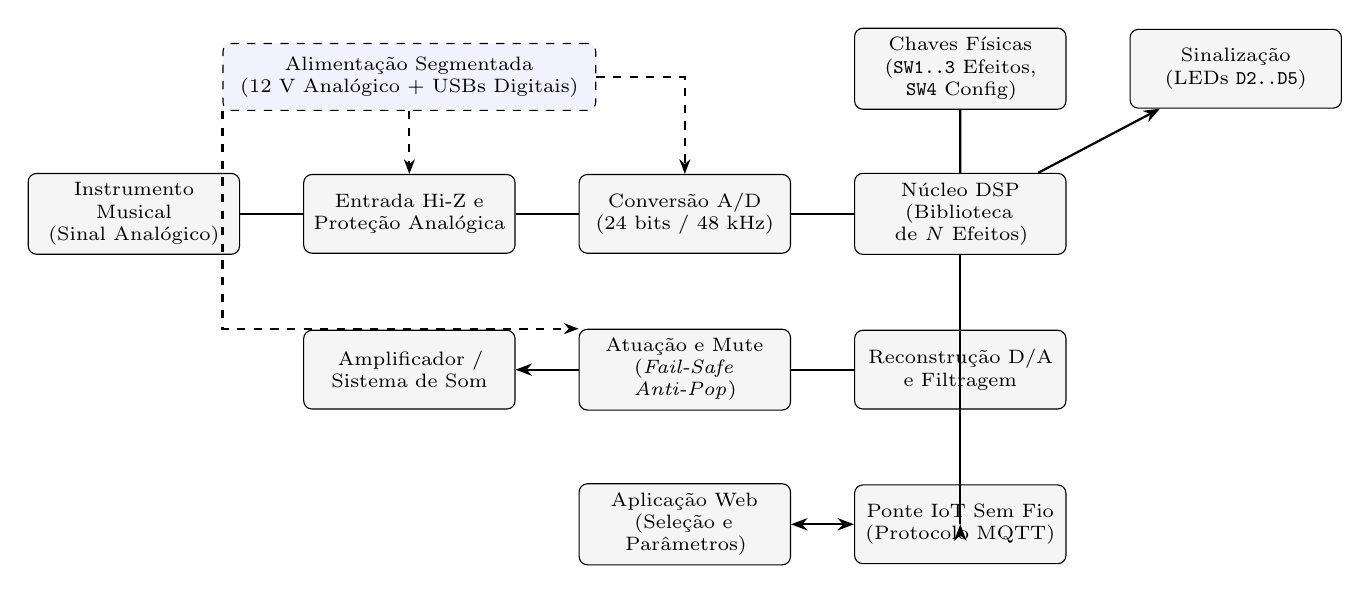
\begin{tikzpicture}[
    node distance=0.7cm and 0.8cm,
    blk/.style={rectangle, draw=black, rounded corners=3pt, minimum height=1.0cm, text width=2.45cm, align=center, font=\scriptsize, fill=gray!8},
    psu/.style={rectangle, draw=black, dashed, rounded corners=3pt, minimum height=0.85cm, text width=4.5cm, align=center, font=\scriptsize, fill=blue!5},
    arr/.style={-{Stealth[scale=0.9]}, thick},
    biarr/.style={{Stealth[scale=0.9]}-{Stealth[scale=0.9]}, thick},
    darr/.style={-{Stealth[scale=0.8]}, dashed, thick}
  ]
    \node[blk] (inst) {Instrumento Musical\\(Sinal Analógico)};
    \node[blk, right=of inst] (in) {Entrada Hi-Z e\\Proteção Analógica};
    \node[blk, right=of in] (adc) {Conversão A/D\\(24 bits / 48 kHz)};
    \node[blk, right=of adc] (dsp) {Núcleo DSP\\(Biblioteca de $N$ Efeitos)};
    \node[blk, below=0.95cm of dsp] (dac) {Reconstrução D/A\\e Filtragem};
    \node[blk, left=of dac] (act) {Atuação e Mute\\(\textit{Fail-Safe Anti-Pop})};
    \node[blk, left=of act] (amp) {Amplificador /\\Sistema de Som};
    \node[blk, above=0.8cm of dsp] (uiin) {Chaves Físicas\\(\texttt{SW1..3} Efeitos, \texttt{SW4} Config)};
    \node[blk, right=of uiin] (uiout) {Sinalização\\(LEDs \texttt{D2..D5})};
    \node[blk, below=0.95cm of dac] (comm) {Ponte IoT Sem Fio\\(Protocolo MQTT)};
    \node[blk, left=of comm] (app) {Aplicação Web\\(Seleção e Parâmetros)};
    \node[psu, above=0.8cm of in] (psu) {Alimentação Segmentada\\(12 V Analógico + USBs Digitais)};
    \draw[arr] (inst) -- (in) -- (adc) -- (dsp) -- (dac) -- (act) -- (amp);
    \draw[arr] (uiin) -- (dsp) -- (uiout);
    \draw[arr] (dsp) |- (comm);
    \draw[biarr] (comm) -- (app);
    \draw[darr] (psu) -- (in);
    \draw[darr] (psu) -| (adc);
    \draw[darr] (psu.south west) |- (act.north west);
  \end{tikzpicture}
  \fonte{Elaborado pelos autores (2026).}
\end{figure}

\section{Arquitetura Preliminar}
A Figura~\ref{fig:arquitetura} detalha os módulos digitais (\texttt{STM32H723VG}, \texttt{CS4272}, \texttt{ESP32}) e a infraestrutura analógica de suporte (\texttt{TL072}, clamp do ADC, isolador \texttt{ISO7721DR}, supervisão \texttt{TL431ACZ} e relé \texttt{K1}).
\begin{figure}[htbp]
  \centering
  \caption{Arquitetura técnica preliminar da pedaleira \texttt{PED-DIGITAL}.}
  \label{fig:arquitetura}
  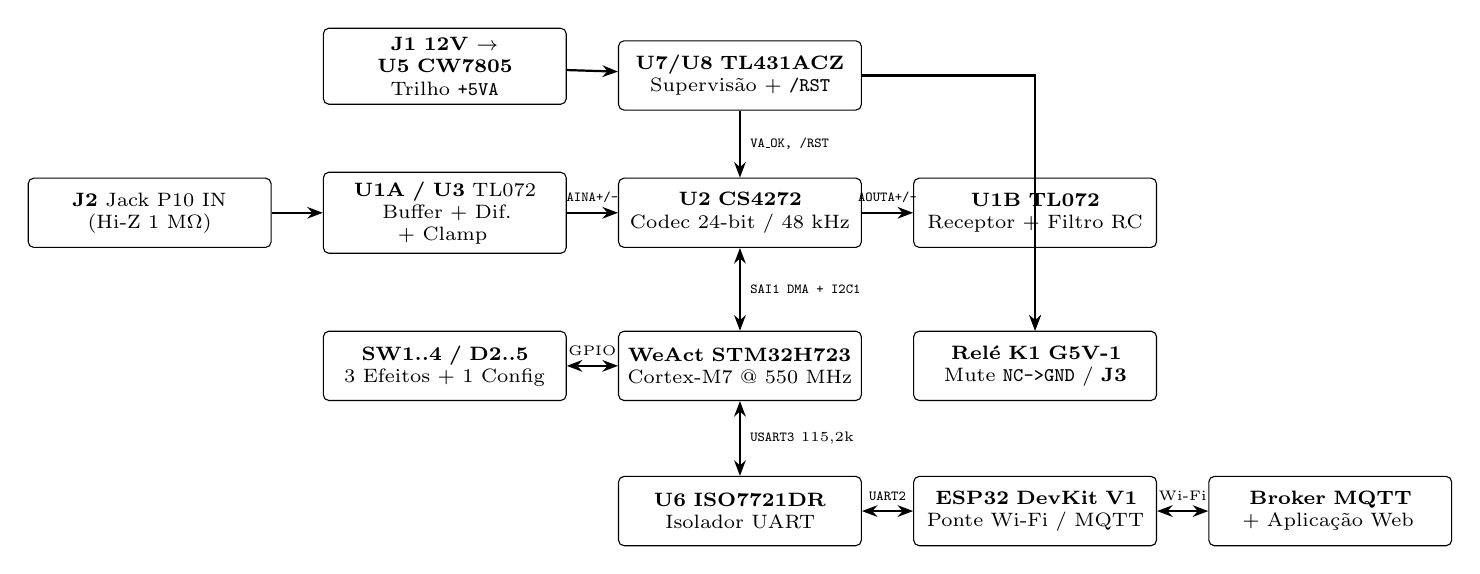
\begin{tikzpicture}[
    node distance=0.55cm and 0.65cm,
    mod/.style={rectangle, draw=black, rounded corners=2pt, minimum height=0.88cm, text width=2.85cm, align=center, font=\scriptsize, fill=white},
    arr/.style={-{Stealth[scale=0.85]}, thick},
    biarr/.style={{Stealth[scale=0.85]}-{Stealth[scale=0.85]}, thick}
  ]
    \node[mod] (j2) {\textbf{J2} Jack P10 IN\\(Hi-Z $1\text{ M}\Omega$)};
    \node[mod, right=of j2] (u1a) {\textbf{U1A / U3} TL072\\Buffer + Dif. + Clamp};
    \node[mod, right=of u1a] (codec) {\textbf{U2 CS4272}\\Codec 24-bit / 48~kHz};
    \node[mod, right=of codec] (u1b) {\textbf{U1B TL072}\\Receptor + Filtro RC};
    \node[mod, below=1.05cm of codec] (stm) {\textbf{WeAct STM32H723}\\Cortex-M7 @ 550~MHz};
    \node[mod, left=of stm] (sw) {\textbf{SW1..4 / D2..5}\\3 Efeitos + 1 Config};
    \node[mod, below=0.95cm of stm] (iso) {\textbf{U6 ISO7721DR}\\Isolador UART};
    \node[mod, right=of iso] (esp) {\textbf{ESP32 DevKit V1}\\Ponte Wi-Fi / MQTT};
    \node[mod, right=of esp] (broker) {\textbf{Broker MQTT}\\+ Aplicação Web};
    \node[mod, below=1.05cm of u1b] (k1) {\textbf{Relé K1 G5V-1}\\Mute \texttt{NC->GND} / \textbf{J3}};
    \node[mod, above=0.85cm of u1a] (cw) {\textbf{J1 12V} $\rightarrow$ \textbf{U5 CW7805}\\Trilho \texttt{+5VA}};
    \node[mod, above=0.85cm of codec] (sup) {\textbf{U7/U8 TL431ACZ}\\Supervisão + \texttt{/RST}};
    \draw[arr] (j2) -- (u1a);
    \draw[arr] (u1a) -- node[above,font=\tiny]{\texttt{AINA+/-}} (codec);
    \draw[arr] (codec) -- node[above,font=\tiny]{\texttt{AOUTA+/-}} (u1b);
    \draw[arr] (u1b) -- (k1);
    \draw[biarr] (codec) -- node[right,font=\tiny]{\texttt{SAI1 DMA + I2C1}} (stm);
    \draw[biarr] (sw) -- node[above,font=\tiny]{GPIO} (stm);
    \draw[biarr] (stm) -- node[right,font=\tiny]{\texttt{USART3} 115,2k} (iso);
    \draw[biarr] (iso) -- node[above,font=\tiny]{\texttt{UART2}} (esp);
    \draw[biarr] (esp) -- node[above,font=\tiny]{Wi-Fi} (broker);
    \draw[arr] (cw) -- (sup);
    \draw[arr] (sup) -- node[right,font=\tiny]{\texttt{VA\_OK, /RST}} (codec);
    \draw[arr] (sup) -| (k1);
  \end{tikzpicture}
  \fonte{Elaborado pelos autores (2026).}
\end{figure}

\section{Divisão em Subsistemas}
O sistema foi particionado em sete subsistemas modulares (Tabela~\ref{tab:subsistemas}).
\begin{table}[htbp]\centering\caption{Divisão do projeto em subsistemas e responsáveis.}\label{tab:subsistemas}
  \scriptsize
  \setlength{\tabcolsep}{3.5pt}
  \begin{tabularx}{\textwidth}{L{3.1cm}L{4.8cm}L{4.0cm}Y}
    \toprule
    \textbf{Subsistema} & \textbf{Função Principal} & \textbf{Componentes / Módulos} & \textbf{Responsável} \\
    \midrule
    \textbf{SS01 -- Processamento DSP} & Motor \texttt{SAI1 DMA}, biblioteca expansível, mapeamento dinâmico e \textit{crossfade}. & \texttt{STM32H723VG}, \texttt{DspEngine}, \texttt{DspOverdrive/EQ/Delay}. & João Paulo / Isabelle \\
    \textbf{SS02 -- Web e MQTT} & Ponte UART isolada (\texttt{CRC-8}), cliente MQTT e aplicação Web de configuração. & \texttt{ESP32 DevKit V1}, \texttt{ISO7721DR}, App Web + Broker MQTT. & Isabelle / João Paulo \\
    \textbf{SS03 -- Interface Física} & Leitura das chaves configuráveis (\texttt{SW1..SW3}), chave Config (\texttt{SW4}) e LEDs. & \texttt{SW1..SW4} (\texttt{MTS-102}), LEDs \texttt{D2..D5}, resistores $330\text{ }\Omega$. & Arthur Ramalho \\
    \textbf{SS04 -- Codec de Áudio} & Amostragem e reconstrução em 24~bits / 48~kHz via I2S e I2C. & \texttt{U2 CS4272} (TSSOP-28 em adaptador) e filtros. & Arthur Ramalho \\
    \textbf{SS05 -- Analógico e Mute} & Buffer Hi-Z, driver diferencial com clamp ativo, filtro RC e relé \textit{anti-pop}. & \texttt{J2}, \texttt{J3}, \texttt{U1/U3 TL072}, clamp \texttt{Q9..Q14}, relé \texttt{K1}. & Rodrigues / Arthur \\
    \textbf{SS06 -- Alimentação} & Entrada \texttt{12 V DC}, regulação \texttt{+5VA} (\texttt{CW7805}), USBs isoladas e supervisão. & \texttt{J1}, \texttt{F1}, \texttt{D1}, \texttt{U5}, \texttt{U7/U8 TL431}, reset \texttt{/RST}. & Rodrigues Matheus \\
    \textbf{SS07 -- Estrutura e Testes} & Placa perfurada ilhada, pontos de teste \texttt{TP1..TP11} e gabinete 3D. & Placa $145\times 95\text{ mm}$, \texttt{TP1..TP11}, gabinete STL. & Toda a equipe \\
    \bottomrule
  \end{tabularx}
  \fonte{Elaborado pelos autores (2026).}
\end{table}

\section{Seleção e Justificativa dos Componentes}
A lista de materiais consolidada no KiCad soma \textbf{183 componentes} (Tabela~\ref{tab:bom}).
\begin{table}[htbp]\centering\caption{Resumo da lista de materiais (BOM consolidada, 183 itens).}\label{tab:bom}
  \footnotesize
  \setlength{\tabcolsep}{3.5pt}
  \begin{tabularx}{\textwidth}{L{2.5cm}L{3.8cm}C{0.8cm}Y L{1.8cm}L{1.7cm}}
    \toprule
    \textbf{Grupo} & \textbf{Referências} & \textbf{Qtd.} & \textbf{Função} & \textbf{Encaps.} & \textbf{Situação} \\
    \midrule
    \textbf{MCU DSP} & \texttt{WeAct STM32H723VG V1.2} & 1 & Núcleo DSP em tempo real (550~MHz) & Módulo 2x22 & Em posse \\
    \textbf{Módulo IoT} & \texttt{ESP32 DevKit V1 (WROOM)} & 1 & Wi-Fi e ponte MQTT & DevKit 30p & Em posse \\
    \textbf{Codec Áudio} & \texttt{Cirrus Logic CS4272} & 1 & ADC/DAC 24~bits / 48~kHz (114~dB) & TSSOP-28+ad. & Em posse \\
    \textbf{Amp-Ops} & \texttt{U1, U3 (TL072)} & 2 & Buffer Hi-Z e estágio diferencial & DIP-8 & Em posse \\
    \textbf{Regulador} & \texttt{U5 (CW7805)} & 1 & Trilho analógico \texttt{+5VA} do codec & TO-220 & Em posse \\
    \textbf{Isolador} & \texttt{U6 (TI ISO7721DR)} & 1 & Isolação UART \texttt{STM32 <-> ESP32} & SOIC-8+ad. & Adquirir \\
    \textbf{Supervisores} & \texttt{U7, U8 (TL431ACZ)} & 2 & Supervisão \texttt{+5VA} e UVLO \texttt{12 V} & TO-92-3 & Adquirir \\
    \textbf{Relé Mute} & \texttt{K1 (Omron G5V-1-DC12)} & 1 & Aterramento \texttt{NC->GND} anti-pop & DIP-6 THT & Adquirir \\
    \textbf{Chaves/LEDs} & \texttt{SW1..4 (MTS-102)}, \texttt{D2..5} & 8 & 3 efeitos + 1 Modo Config + LEDs & THT & Adquirir \\
    \textbf{Discretos} & \texttt{Q1..22}, diodos, \texttt{J1..5}, \texttt{R1..75}, \texttt{C1..49}, \texttt{TP1..11} & 165 & Clamp ativo, lógica de mute, filtros RC e pontos de teste & THT / Axial & Adquirir \\
    \bottomrule
  \end{tabularx}
  \fonte{Elaborado pelos autores (2026).}
\end{table}

As escolhas principais seguiram critérios técnicos mensuráveis \cite{ifpb2026roteiro}. O \textbf{\texttt{STM32H723VG}} \cite{st2023stm32h723, weact2022stm32h723} fornece FPU nativa a 550~MHz, \texttt{SAI1 DMA} e 564~KB de SRAM interna, com folga de CPU acima de $70\%$. O codec \textbf{\texttt{CS4272}} \cite{cirrus2015cs4272} entrega faixa dinâmica de 114~dB e entradas e saídas diferenciais. O módulo \textbf{\texttt{ESP32-WROOM-32}} \cite{espressif2023esp32} isola o tráfego Wi-Fi e MQTT em FreeRTOS fora do laço de áudio. A infraestrutura analógica usa \textbf{\texttt{TL072}} \cite{ti2015tl072} na entrada JFET Hi-Z, \textbf{\texttt{ISO7721DR}} \cite{ti2020iso7721} contra retorno de corrente entre portas USB, \textbf{\texttt{TL431ACZ}} \cite{ti2018tl431} na supervisão e o relé \textbf{\texttt{G5V-1-DC12}} \cite{omron2020g5v1} para \textit{mute} físico sem alimentação.

\section{Consulta aos Datasheets}
A Tabela~\ref{tab:datasheets} consolida os parâmetros extraídos dos manuais oficiais.
\begin{table}[htbp]\centering\caption{Parâmetros principais extraídos dos datasheets oficiais.}\label{tab:datasheets}
  \scriptsize
  \setlength{\tabcolsep}{3.5pt}
  \begin{tabularx}{\textwidth}{L{2.1cm}L{1.8cm}L{2.3cm}L{2.2cm}L{2.6cm}Y}
    \toprule
    \textbf{Componente} & \textbf{Fabricante} & \textbf{Alimentação} & \textbf{Consumo} & \textbf{Desempenho} & \textbf{Cuidado de Projeto} \\
    \midrule
    \textbf{STM32H723VG} & STMicro. & 3,3~V (buck WeAct) & $\le 329{,}4\text{ mA}$ & 550~MHz, FPU, SAI1 & Conferir capacidade do buck \texttt{U2}. \\
    \textbf{CS4272} & Cirrus Logic & VA: 5~V; VD/VL: 3,3~V & IA: 53~mA; ID+IL: 28~mA & 114~dB DR; 24b/48k & Limite estrito em \texttt{AIN}: $[\text{GND}-0{,}3, \text{VA}+0{,}3]$~V. \\
    \textbf{ESP32} & Espressif & 3,3~V (USB 5~V) & $\sim 80\text{ mA}$ (pico 500~mA) & Wi-Fi; UART 115,2k & Confirmar \texttt{WROOM} (\texttt{GPIO16/17} livres). \\
    \textbf{TL072} & Texas Inst. & \texttt{+RAW} ($\sim 11{,}5\text{ V}$) & $\sim 4\text{ mA}$ / CI & $R_{\text{in}} \sim 10^{12}\text{ }\Omega$ & Sinal $< 1{,}4\text{ V}_{\text{p}}$ e carga $\ge 10\text{ k}\Omega$. \\
    \textbf{ISO7721DR} & Texas Inst. & Dual 3,3~V / 3,3~V & $\sim 4\text{ mA}$ / lado & Até 100~Mbps & Evitar variante \texttt{F}; manter \textit{default HIGH}. \\
    \textbf{TL431ACZ} & Texas Inst. & Shunt 2,5--36~V & $I_{k,\min} \le 1\text{ mA}$ & $V_{\text{ref}} = 2{,}495\text{ V} \pm 1\%$ & Garantir corrente de cátodo $\ge 1\text{ mA}$. \\
    \textbf{G5V-1-DC12} & Omron & Bobina 12~V DC & 12,5~mA @ 12~V & Op./lib. $\le 5\text{ ms}$ & Requer diodo \textit{flyback} \texttt{D16}. \\
    \bottomrule
  \end{tabularx}
  \fonte{Compilado de \cite{st2023stm32h723, cirrus2015cs4272, espressif2023esp32, ti2015tl072, ti2018tl431, ti2020iso7721, omron2020g5v1}.}
\end{table}

\section{Tecnologias de Software}
A Tabela~\ref{tab:soft} resume a pilha de software adotada no firmware e na interface Web/MQTT.
\begin{table}[htbp]\centering\caption{Tecnologias e ferramentas de software empregadas.}\label{tab:soft}
  \footnotesize
  \begin{tabularx}{\textwidth}{L{3.8cm}L{3.9cm}Y}
    \toprule
    \textbf{Tecnologia / Ferramenta} & \textbf{Aplicação} & \textbf{Justificativa Técnica} \\
    \midrule
    \textbf{C++17 + CMSIS-DSP} & Firmware DSP na \texttt{STM32H723VG} & Zero alocação dinâmica no loop de áudio e uso de FPU/SIMD. \\
    \textbf{FreeRTOS / ESP-IDF} & Firmware ponte no \texttt{ESP32} & Execução concorrente de Wi-Fi, cliente MQTT e UART sem bloqueios. \\
    \textbf{Aplicação Web + MQTT} & Configuração pelo usuário & Seleciona efeitos da biblioteca, mapeia às chaves e ajusta parâmetros. \\
    \textbf{Protocolo UART CRC-8} & Ligação \texttt{STM32 <-> ESP32} & Quadro binário compacto dispensando \textit{parsing} JSON na STM32. \\
    \textbf{KiCad 10 + \texttt{ngspice}} & Esquemáticos e simulações & Fluxo aberto para verificação ERC e validação analógica pré-bancada. \\
    \bottomrule
  \end{tabularx}
  \fonte{Elaborado pelos autores (2026).}
\end{table}

\section{Fluxo de Dados e Sistema de Alimentação}
O sistema coordena dois fluxos principais sobre uma alimentação segmentada:
\begin{enumerate}
  \item \textbf{Áudio em Tempo Real}: O sinal entra em \texttt{J2} ($1\text{ M}\Omega$), passa pelo estágio diferencial \texttt{TL072} protegido e é digitalizado pelo \texttt{CS4272} (24~bits / 48~kHz). O barramento \texttt{SAI1} com \texttt{DMA} duplo entrega blocos à \texttt{STM32H723VG}, que processa os efeitos ativos atribuídos às chaves (\textit{Overdrive}, EQ 3 bandas, \textit{Delay} ou novos módulos) com \textit{crossfade anti-pop} e devolve o sinal a \texttt{J3}.
  \item \textbf{Configuração via Rede (Web $\leftrightarrow$ MQTT $\leftrightarrow$ Chaves)}: Na aplicação Web, o músico atribui efeitos às chaves físicas (\texttt{SW1..SW3}) e ajusta parâmetros. Os comandos trafegam via MQTT ao \texttt{ESP32} e seguem pela UART isolada (\texttt{ISO7721DR}) à \texttt{STM32}. A chave \texttt{SW4} habilita o Modo de Configuração no painel. Durante a execução, \texttt{SW1..SW3} ligam ou contornam os efeitos mapeados e sincronizam o estado com a Web.
  \item \textbf{Alimentação e Proteção (Suporte)}: Fonte externa de \textbf{12~V~DC / 1,5~A} alimenta o estágio analógico e gera \texttt{+5VA} via \texttt{CW7805} ($< 65\text{ mA}$) para o codec. As placas \texttt{STM32} e \texttt{ESP32} usam USBs independentes em bancada, isoladas pelo \texttt{ISO7721DR}. Supervisores \texttt{TL431ACZ} travam o reset do codec e aterram a saída via relé \texttt{K1} (\texttt{NC -> GND}) em qualquer subtensão.
\end{enumerate}

% ------------------------------------------------------------------------------
\chapter{Projeto Conceitual 3D do Gabinete}
% ------------------------------------------------------------------------------

\section{Especificação Mecânica e Modelagem Paramétrica}
O gabinete paramétrico (\texttt{pedaleira\_gabinete\_3d.stl}, dimensões externas $180{,}0 \times 120{,}0 \times 55{,}0\text{ mm}$, parede $3{,}0\text{ mm}$) foi projetado para abrigar a placa perfurada ($145 \times 95\text{ mm}$) e ser impresso em FDM (PETG ou ABS, camada $0{,}20\text{ mm}$, preenchimento 25\%--30\%, sem suportes). A Tabela~\ref{tab:mapeamento_3d} lista as coordenadas dos controles e conectores.
\begin{table}[htbp]\centering\caption{Mapeamento geométrico dos controles e conectores no gabinete 3D.}\label{tab:mapeamento_3d}
  \footnotesize
  \begin{tabularx}{\textwidth}{L{1.8cm}L{2.8cm}L{3.5cm}L{3.6cm}Y}
    \toprule
    \textbf{Ref.} & \textbf{Componente} & \textbf{Função} & \textbf{Posição $(X, Y, Z)$ (mm)} & \textbf{Furo / Recorte} \\
    \midrule
    \texttt{SW1}+\texttt{D2} & MTS-102 + LED & Efeito Atribuído 1 & $X = -57{,}0$, $Y = -20{,}0 / +6{,}0$ & $\varnothing 6{,}5$ / $\varnothing 5{,}2\text{ mm}$ \\
    \texttt{SW2}+\texttt{D3} & MTS-102 + LED & Efeito Atribuído 2 & $X = -19{,}0$, $Y = -20{,}0 / +6{,}0$ & $\varnothing 6{,}5$ / $\varnothing 5{,}2\text{ mm}$ \\
    \texttt{SW3}+\texttt{D4} & MTS-102 + LED & Efeito Atribuído 3 & $X = +19{,}0$, $Y = -20{,}0 / +6{,}0$ & $\varnothing 6{,}5$ / $\varnothing 5{,}2\text{ mm}$ \\
    \texttt{SW4}+\texttt{D5} & MTS-102 + LED & \textbf{Modo Config (Web/ESP32)} & $X = +57{,}0$, $Y = -20{,}0 / +6{,}0$ & $\varnothing 6{,}5$ / $\varnothing 5{,}2\text{ mm}$ \\
    \texttt{J1} & Jack Barrel & Entrada 12~V DC & $X = -45{,}0, Y = +60{,}0, Z = 24{,}0$ & $\varnothing 11{,}0\text{ mm}$ \\
    \texttt{J2 / J3} & Jacks P10 Mono & \texttt{IN P10} / \texttt{OUT P10} & $X = \pm 90{,}0, Y = 0{,}0, Z = 26{,}0$ & $\varnothing 10{,}5\text{ mm}$ \\
    \texttt{USB1/2} & Recortes USB & \texttt{STM32} / \texttt{ESP32} & $X = 0{,}0 / +45{,}0, Y = +60{,}0, Z = 24{,}0$ & $13{,}0 \times 8{,}0\text{ mm}$ \\
    \bottomrule
  \end{tabularx}
  \fonte{Elaborado pelos autores (2026).}
\end{table}

\section{Renderizações Conceituais do Gabinete}
A Figura~\ref{fig:render1} mostra a perspectiva isométrica externa. A Figura~\ref{fig:render2} apresenta a vista explodida interna dos módulos. A Figura~\ref{fig:render3} detalha o painel superior com \texttt{SW1..SW4} e \texttt{D2..D5}, enquanto a Figura~\ref{fig:render4} exibe as faces laterais e traseira.
\begin{figure}[htbp]\centering\caption{Vista isométrica externa do gabinete conceitual \texttt{PED-DIGITAL}.}\label{fig:render1}
  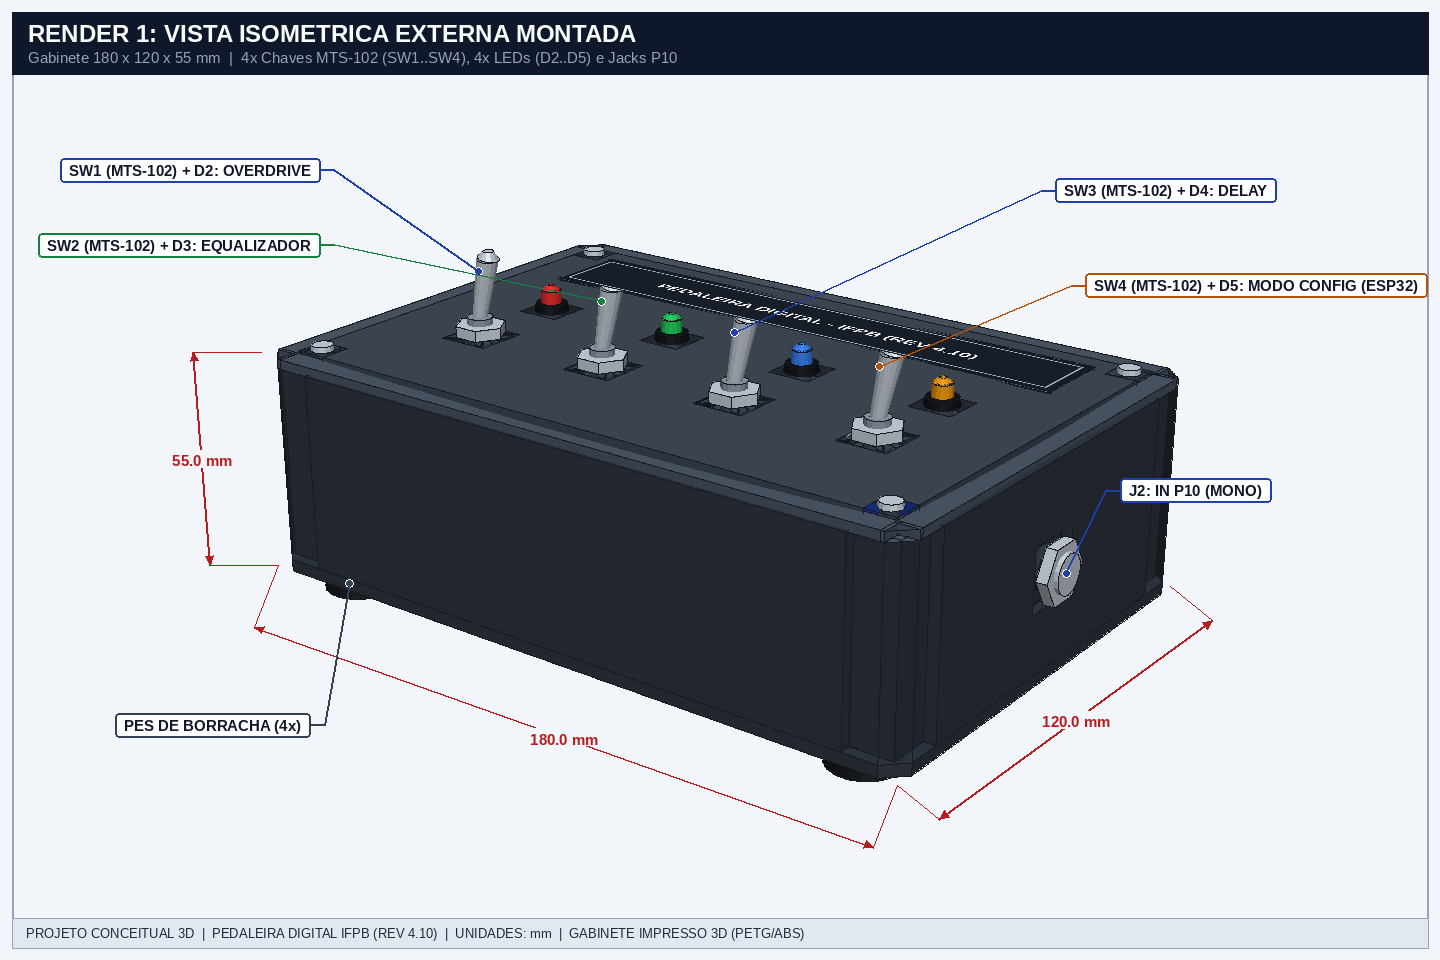
\includegraphics[width=0.84\textwidth]{figuras/render1_isometrica_externa.png}
  \fonte{Elaborado pelos autores (2026).}\end{figure}
\begin{figure}[htbp]\centering\caption{Vista explodida em quatro camadas da montagem interna prevista.}\label{fig:render2}
  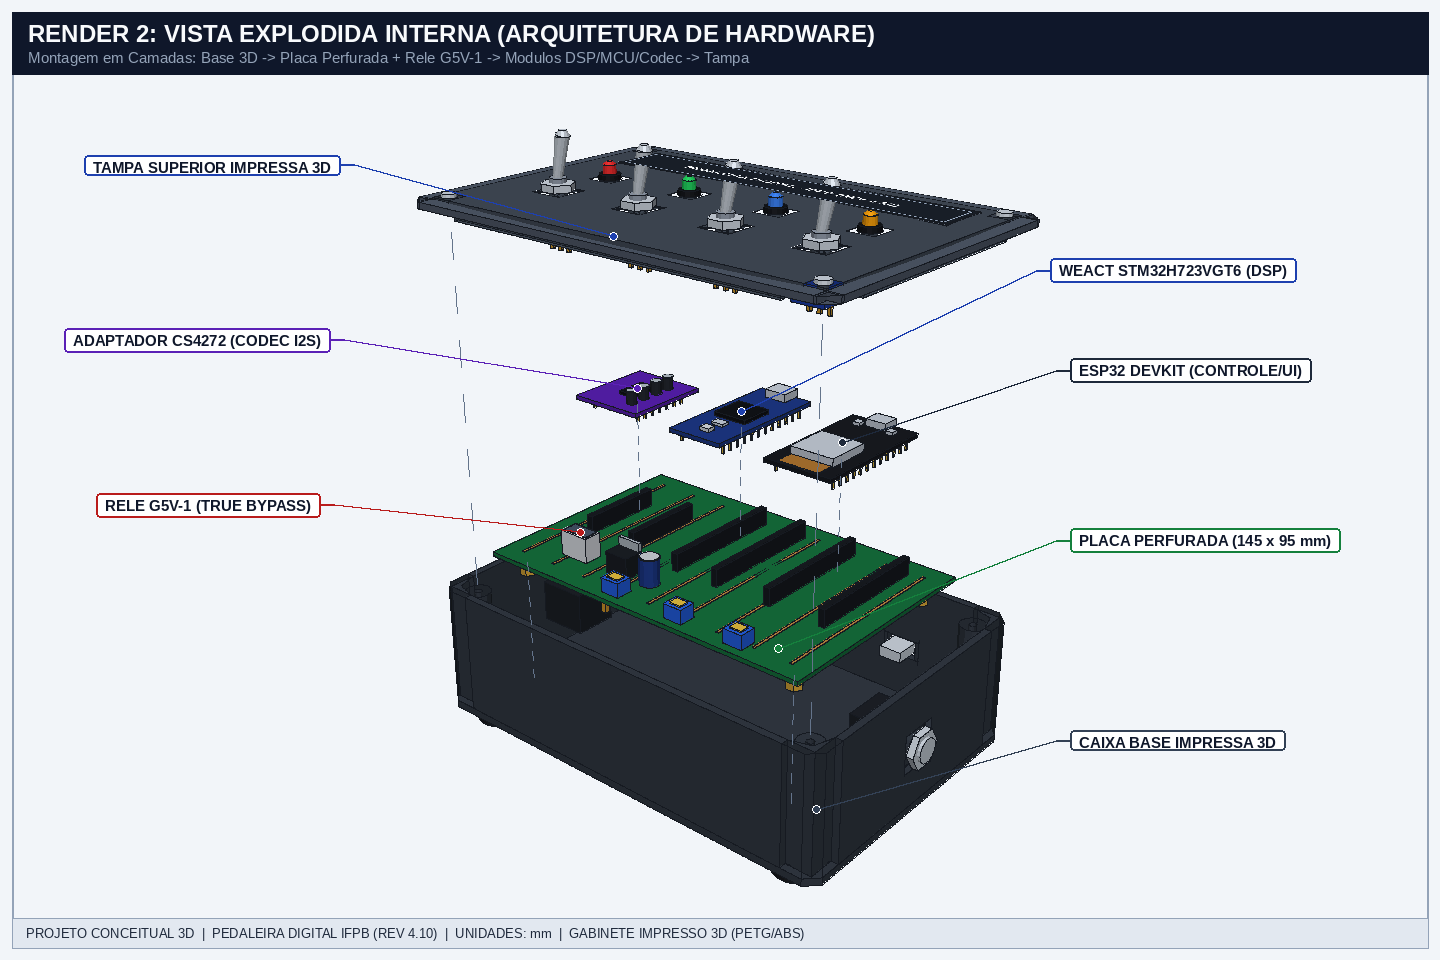
\includegraphics[width=0.84\textwidth]{figuras/render2_vista_explodida_interna.png}
  \fonte{Elaborado pelos autores (2026).}\end{figure}
\begin{figure}[htbp]\centering\caption{Vista ortográfica superior com cotas e disposição de \texttt{SW1..SW4} e \texttt{D2..D5}.}\label{fig:render3}
  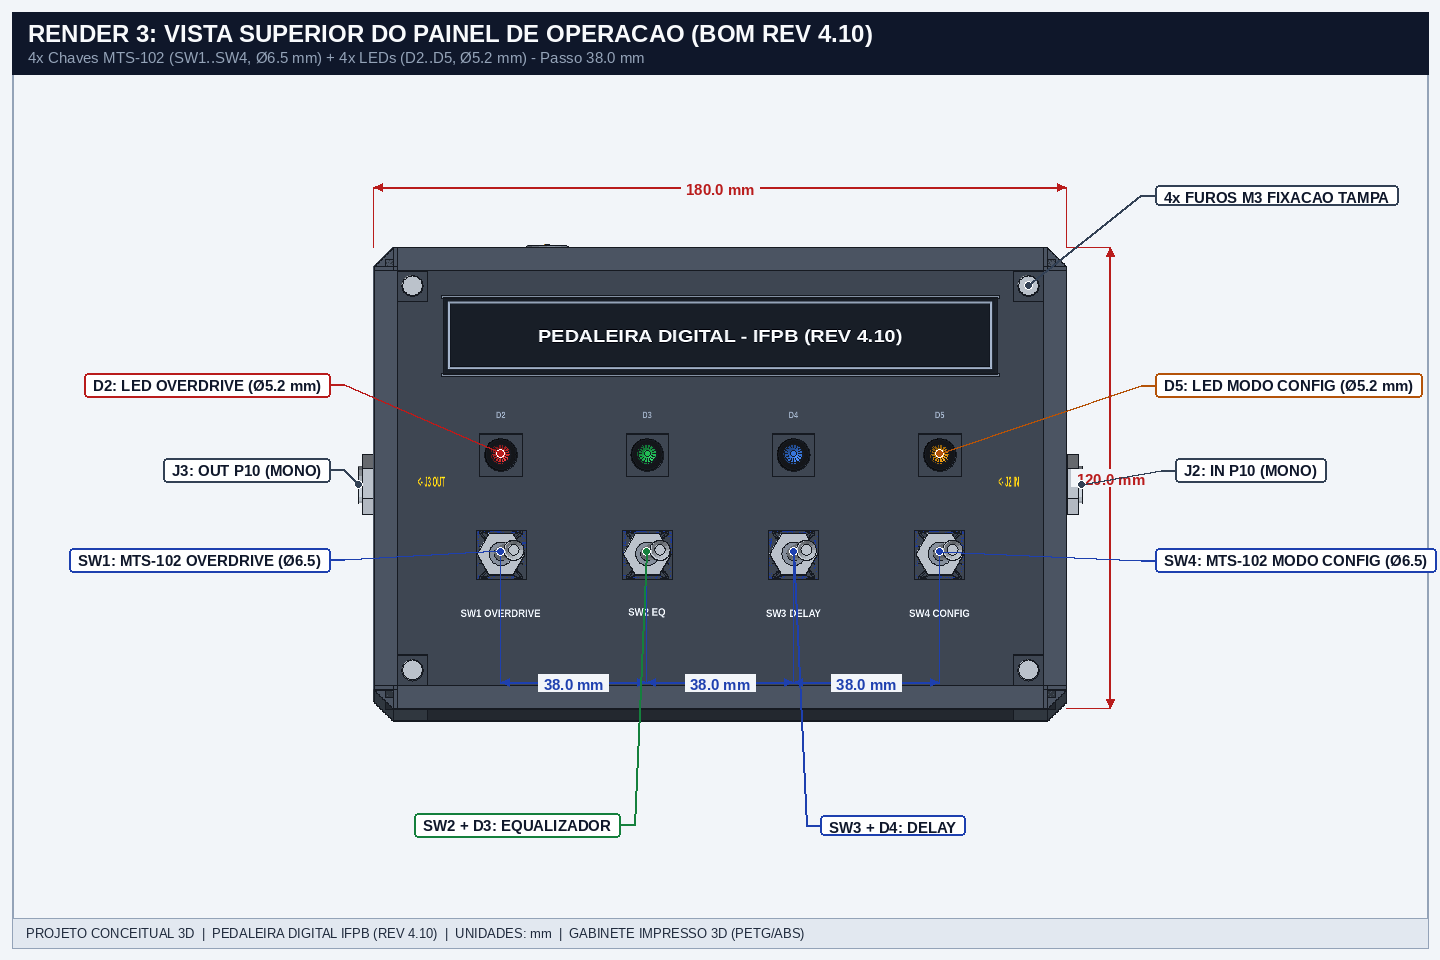
\includegraphics[width=0.84\textwidth]{figuras/render3_painel_superior.png}
  \fonte{Elaborado pelos autores (2026).}\end{figure}
\begin{figure}[htbp]\centering\caption{Vistas ortográficas dos conectores laterais P10 e painel traseiro (12~V DC e USBs).}\label{fig:render4}
  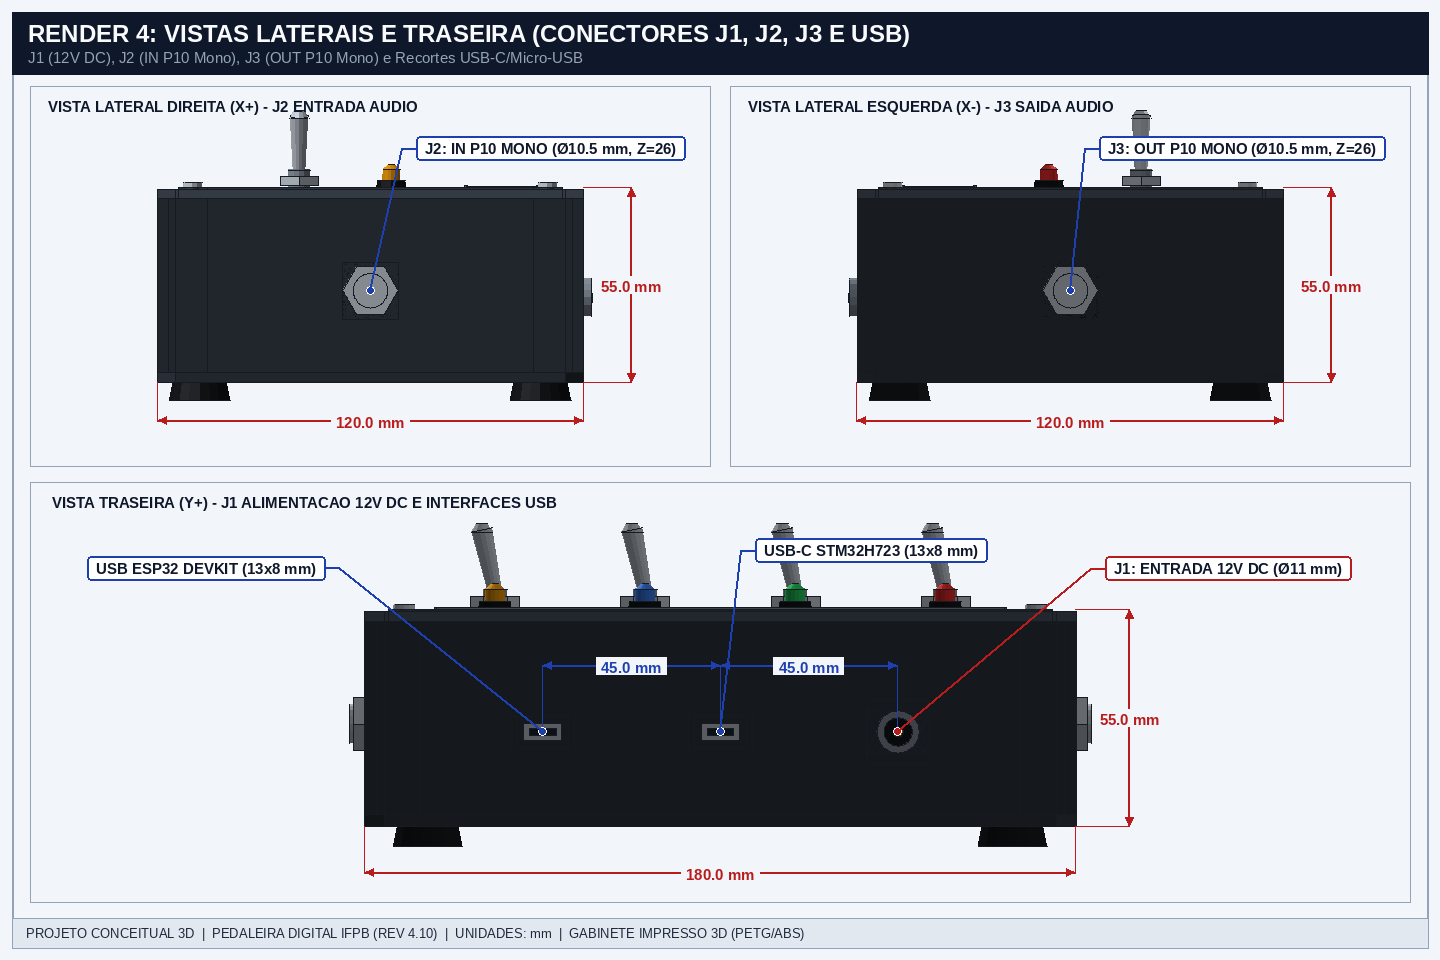
\includegraphics[width=0.84\textwidth]{figuras/render4_conectores_laterais.png}
  \fonte{Elaborado pelos autores (2026).}\end{figure}

\chapter{Simulações Elétricas (SPICE) e Funcionais (DSP)}

\section{Síntese das Simulações Realizadas}
Antes da montagem física, a infraestrutura elétrica de suporte foi validada em 33 cenários SPICE (\texttt{ngspice}) e os algoritmos DSP foram simulados em C++17 a $f_s = 48\text{ kHz}$ (Tabela~\ref{tab:resumo_sim}).
\begin{table}[htbp]\centering\caption{Resumo das simulações elétricas (SPICE) e funcionais (DSP) validadas.}\label{tab:resumo_sim}
  \footnotesize
  \begin{tabularx}{\textwidth}{C{0.8cm}L{3.1cm}L{2.8cm}Y}
    \toprule
    \textbf{\#} & \textbf{Figura} & \textbf{Domínio} & \textbf{Escopo de Verificação} \\
    \midrule
    1 & Figura~\ref{fig:sim1} & SPICE (\texttt{ngspice}) & Partida/colapso (\texttt{0--95 ms}), supervisão \texttt{+5VA}, intertravamento \texttt{/RST} e contenção \texttt{AIN}. \\
    2 & Figura~\ref{fig:sim2} & SPICE (\texttt{ngspice}) & Clamp ativo do ADC (\texttt{Q9..Q14}) vs. Schottky, cantos PVT (0--70\textdegree{}C) e THD. \\
    3 & Figura~\ref{fig:sim3} & SPICE (\texttt{ngspice}) & Mute \textit{anti-pop} por relé \texttt{K1} (\texttt{0--7 s}) e corte rápido na queda de 12~V. \\
    4 & Figura~\ref{fig:sim4} & SPICE (\texttt{ngspice}) & Resposta em frequência (Bode) e \textit{headroom} da cadeia \texttt{TL072}. \\
    5 & Figura~\ref{fig:sim5} & DSP C++17 (48~kHz) & Curva \texttt{SoftLimit}, espectro FFT do \textit{Overdrive} e resposta do EQ 3 bandas. \\
    6 & Figura~\ref{fig:sim6} & DSP C++17 (48~kHz) & Supressão de clique com \textit{crossfade} de potência constante ($\cos/\sin$) vs. corte abrupto. \\
    \bottomrule
  \end{tabularx}
  \fonte{Elaborado pelos autores (2026).}
\end{table}

\section{Validação Elétrica da Infraestrutura Analógica e Proteções (SPICE)}
Os ensaios em \texttt{ngspice} verificaram a resposta dos estágios de suporte:
\begin{itemize}
  \item \textbf{Sequenciamento e Intertravamento (Figura~\ref{fig:sim1})}: O supervisor \texttt{U7} (\texttt{TL431ACZ}) comuta \texttt{VA\_OK} em $4{,}60\text{ V}$/$4{,}52\text{ V}$ (histerese de $85{,}3\text{ mV}$). Sem \texttt{+5VA}, trava \texttt{/RST} em $0{,}024\text{ V}$ e aterra \texttt{AIN} em $\le 0{,}5\text{ mV}$.
  \item \textbf{Clamp Ativo do ADC (Figura~\ref{fig:sim2})}: O clamp compensado por $V_{be}$ (\texttt{Q9..Q14}) mantém \texttt{AINA+/-} dentro de $[+0{,}30\text{ V}, +4{,}99\text{ V}]$ em 0--70\textdegree{}C, com $0{,}000\text{ mA}$ de retorno em \texttt{+5VA} e $\text{THD} = 0{,}00088\%$ a $0\text{ dBFS}$.
  \item \textbf{Mute Anti-Pop a Relé \texttt{K1} (Figura~\ref{fig:sim3})}: A saída permanece em $0{,}0\text{ mV}$ durante os $5{,}90\text{ s}$ iniciais e libera o áudio com transiente de $1{,}23\text{ mV}$ ($< 5\text{ mV}$). Na retirada da fonte, \texttt{K1} aterra \texttt{J3} em $8{,}26\text{ ms}$ com isolação de $-185{,}6\text{ dB}$.
  \item \textbf{Resposta em Frequência e Headroom (Figura~\ref{fig:sim4})}: Resposta plana de 100~Hz a 10~kHz e excursão interna dentro de $[3{,}85\text{ V}, 6{,}65\text{ V}]$ com fonte a $10{,}5\text{ V}$ (margem de $3{,}85\text{ V}$).
\end{itemize}
\begin{figure}[htbp]\centering\caption{Simulação SPICE: sequenciamento de partida, supervisor \texttt{+5VA} e intertravamento \texttt{/RST}.}\label{fig:sim1}
  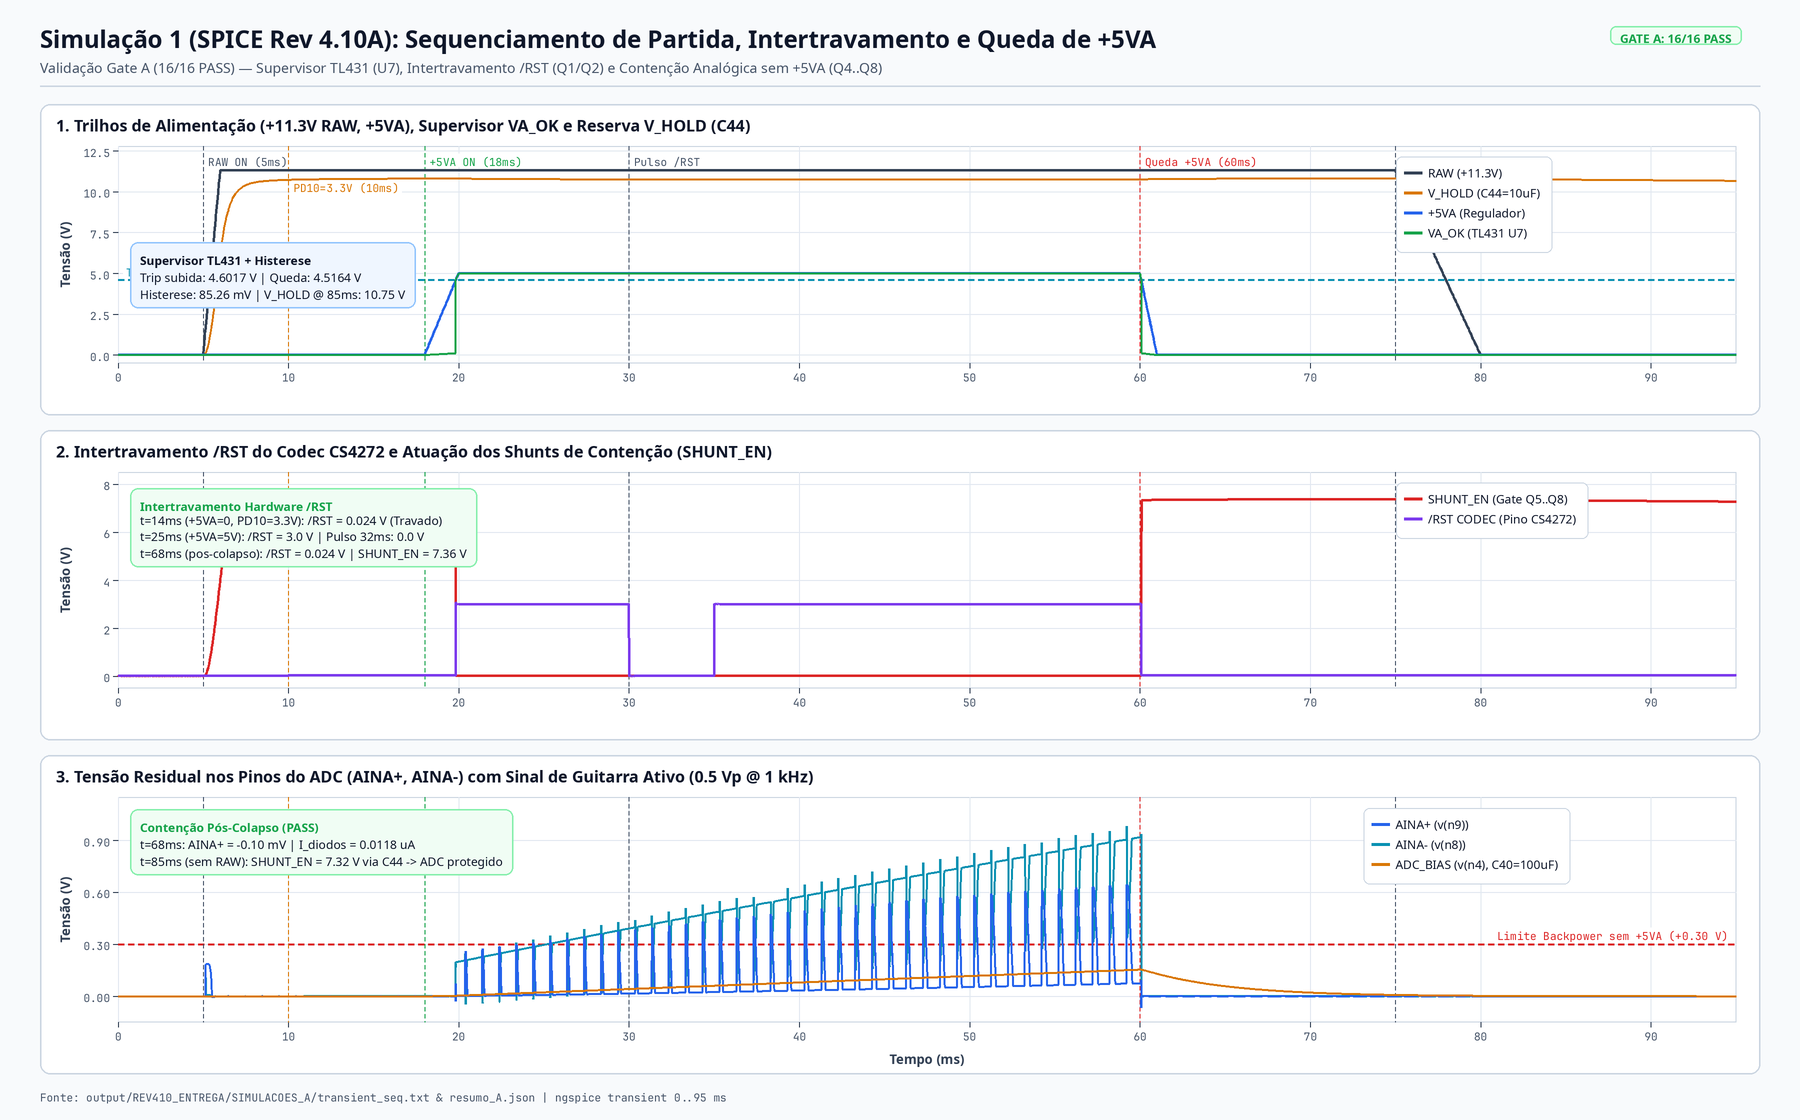
\includegraphics[width=0.88\textwidth]{figuras/sim1_sequenciamento_partida.png}
  \fonte{Elaborado pelos autores (2026).}\end{figure}
\begin{figure}[htbp]\centering\caption{Simulação SPICE: proteção ativa do ADC compensada por $V_{be}$ em cantos PVT e análise THD.}\label{fig:sim2}
  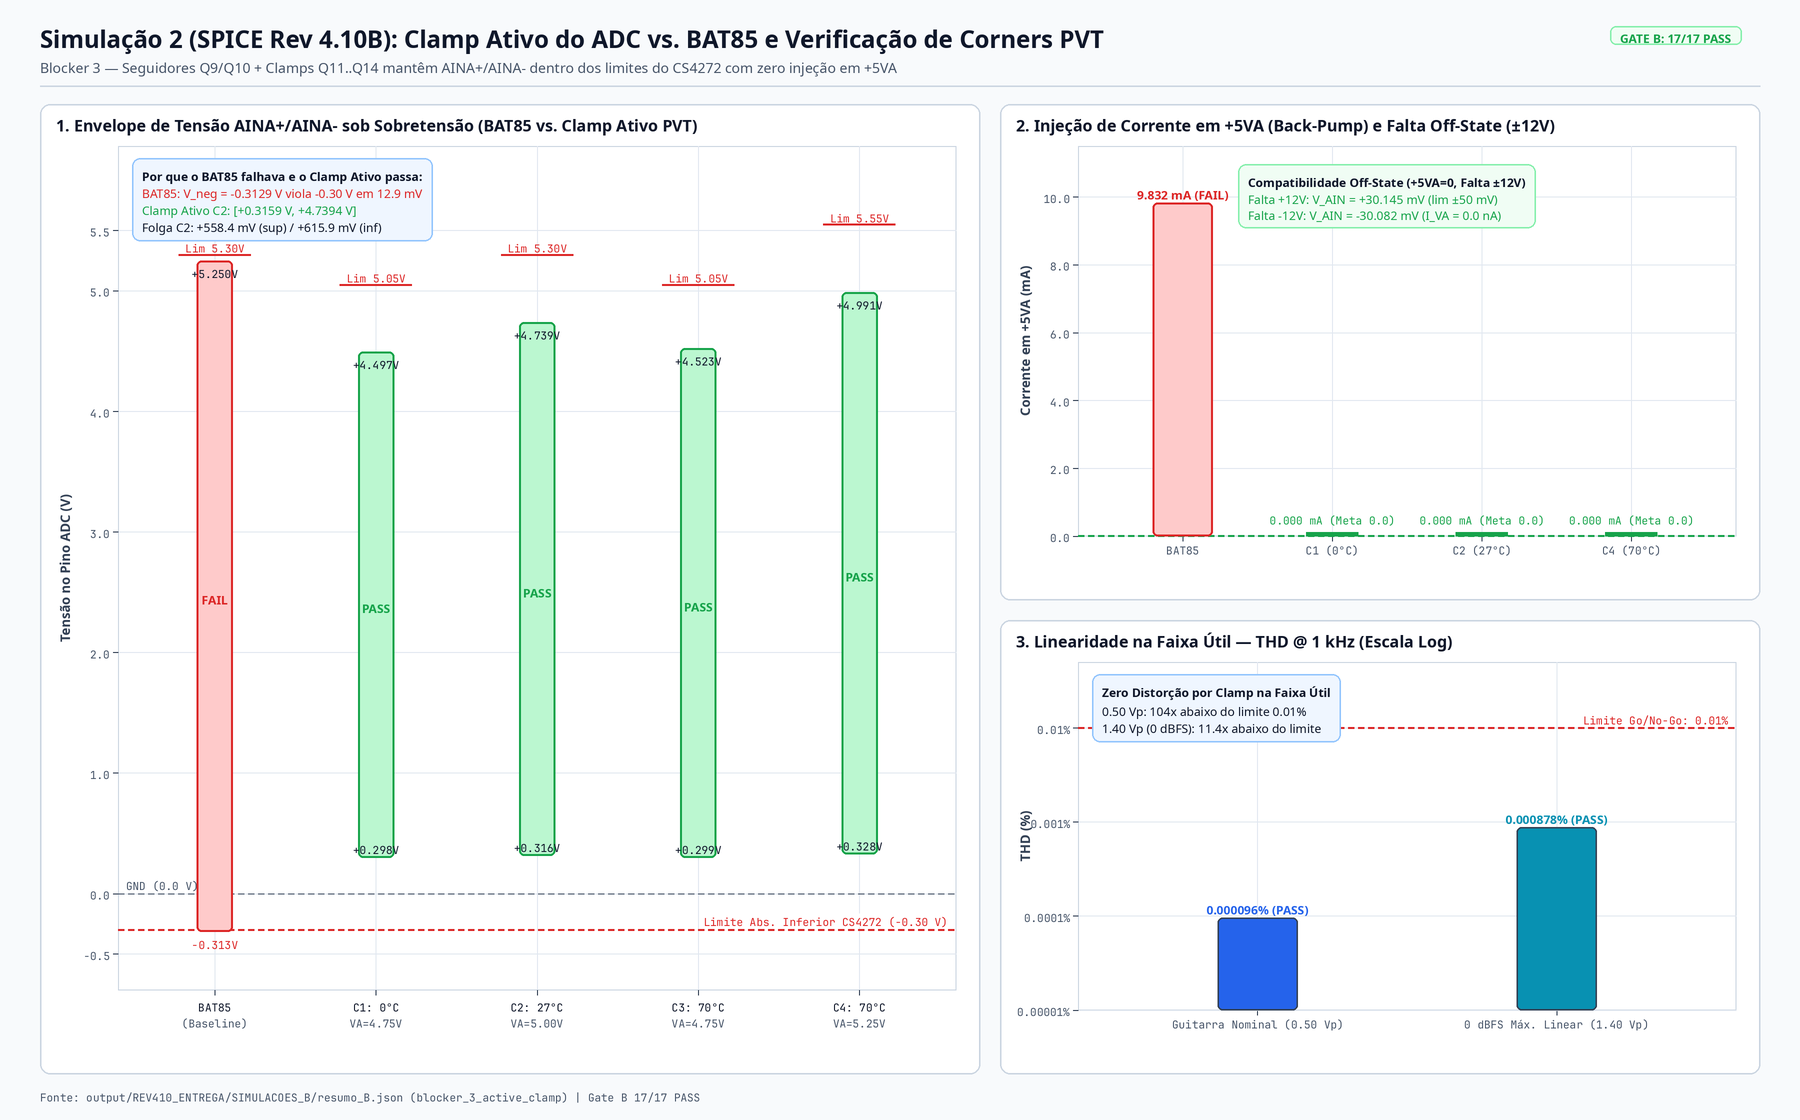
\includegraphics[width=0.88\textwidth]{figuras/sim2_clamp_ativo_adc.png}
  \fonte{Elaborado pelos autores (2026).}\end{figure}
\begin{figure}[htbp]\centering\caption{Simulação SPICE: partida \textit{anti-pop} (0--7~s) e corte rápido de saída pelo relé \texttt{K1}.}\label{fig:sim3}
  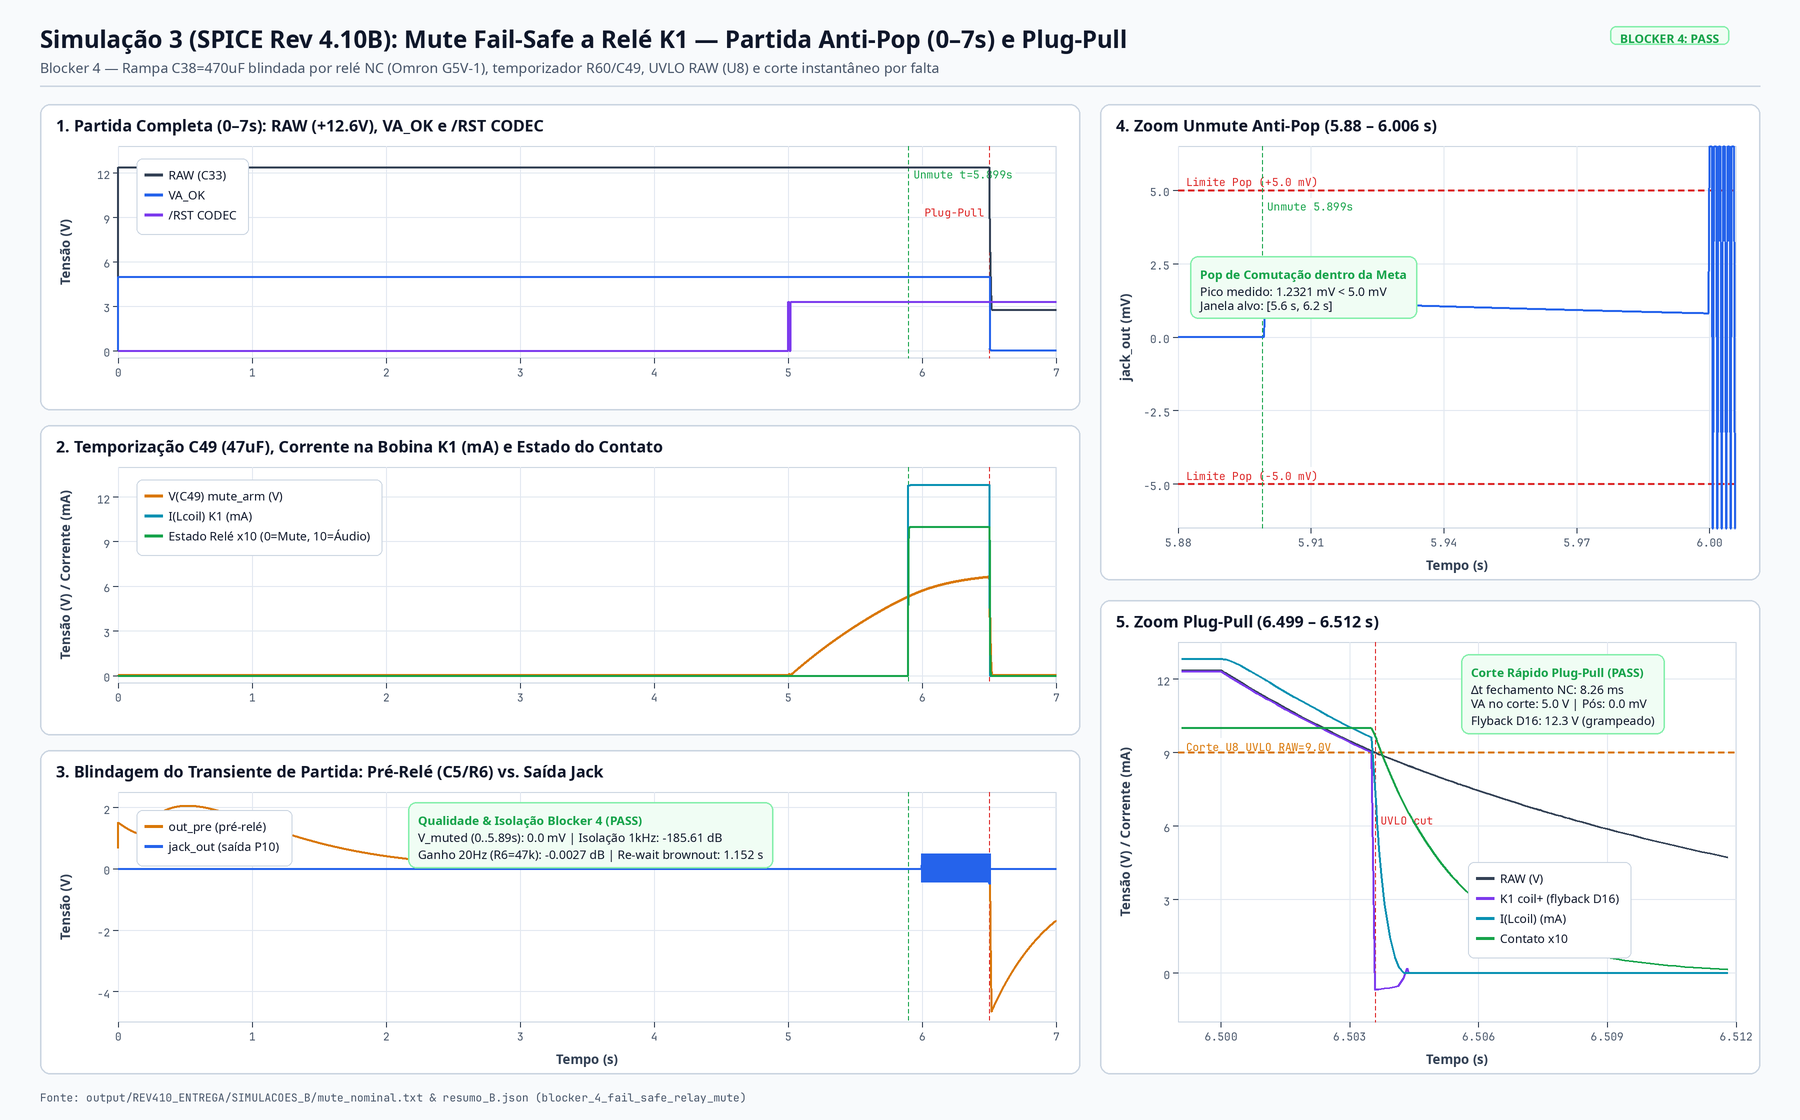
\includegraphics[width=0.88\textwidth]{figuras/sim3_mute_antipop_plugpull.png}
  \fonte{Elaborado pelos autores (2026).}\end{figure}
\begin{figure}[htbp]\centering\caption{Simulação SPICE: diagrama de Bode e margens de \textit{headroom} da cadeia analógica.}\label{fig:sim4}
  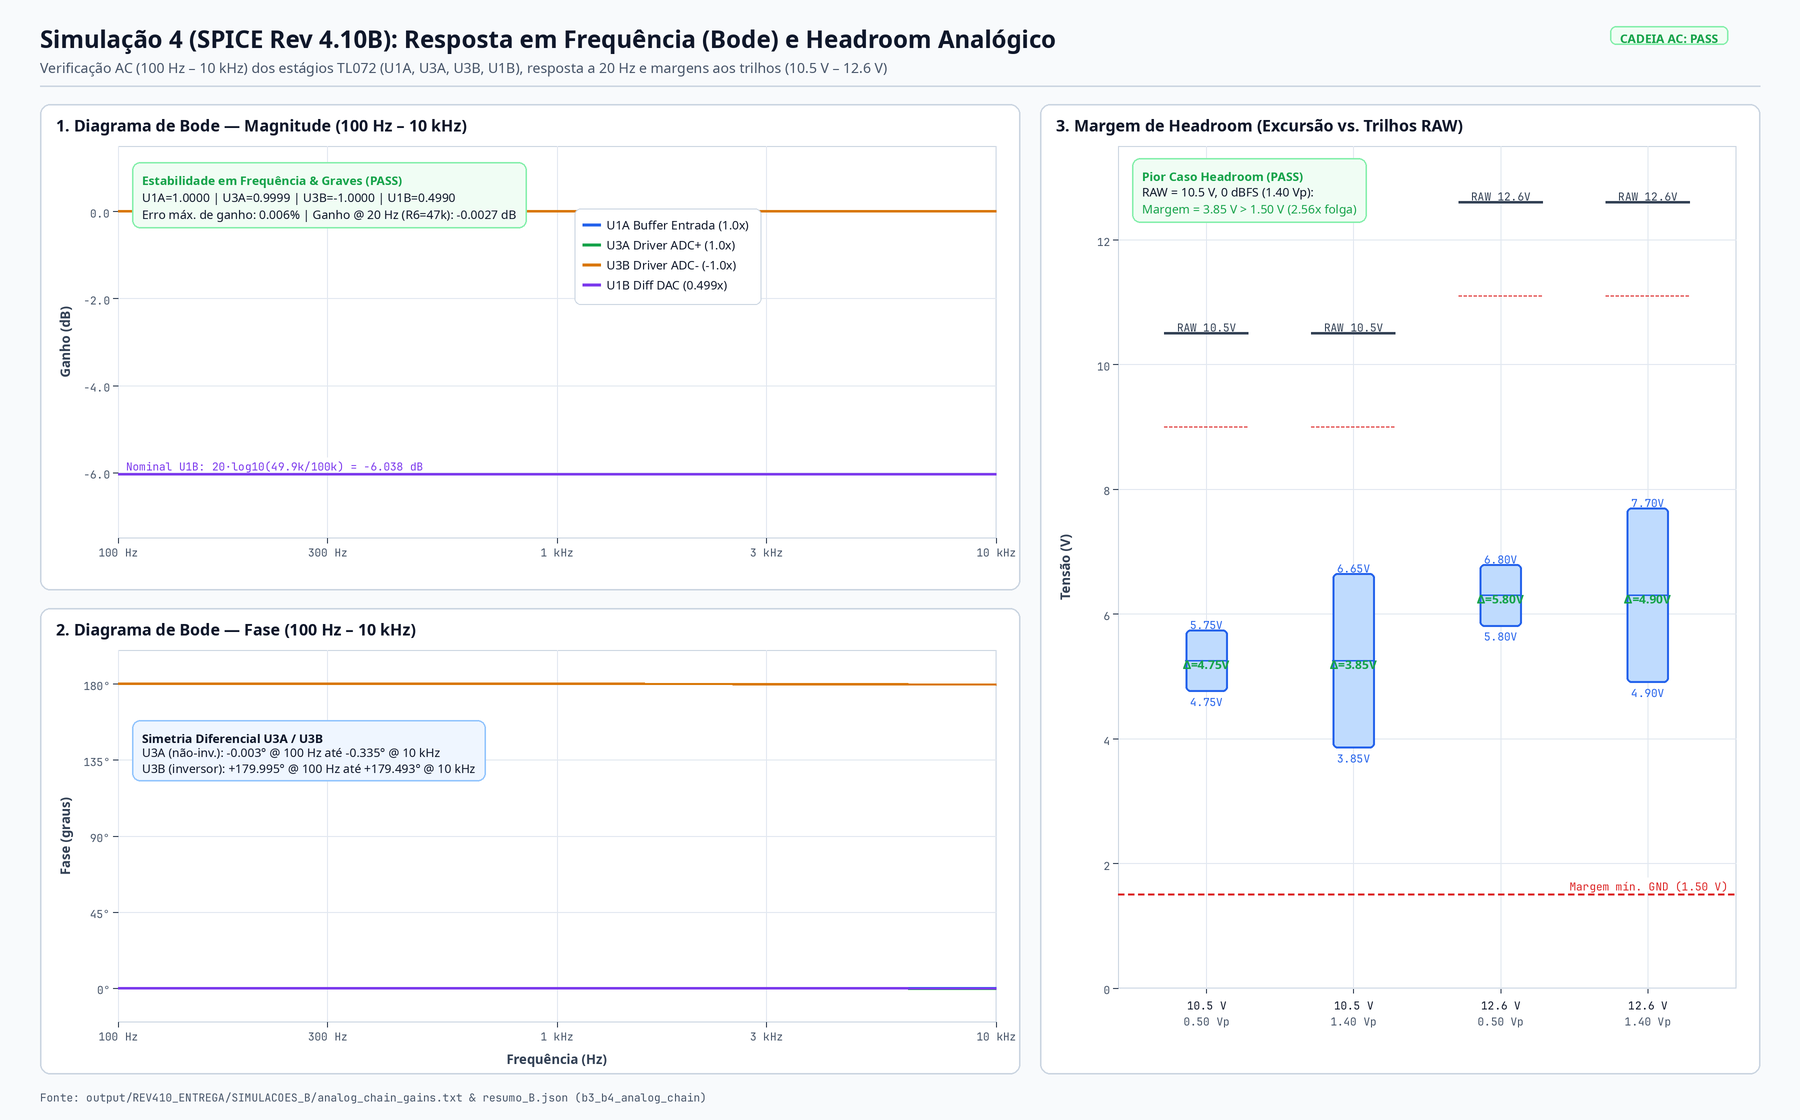
\includegraphics[width=0.88\textwidth]{figuras/sim4_bode_cadeia_analogica.png}
  \fonte{Elaborado pelos autores (2026).}\end{figure}

\section{Validação Funcional dos Algoritmos DSP (C++17, $f_s = 48\text{ kHz}$)}
Os módulos da biblioteca DSP foram validados em C++17 nativo a 48~kHz sem alocação dinâmica:
\begin{itemize}
  \item \textbf{Overdrive e EQ 3 Bandas (Figura~\ref{fig:sim5})}: \texttt{DspOverdrive} combina saturação cúbica \texttt{SoftLimit} e filtro passa-baixas \texttt{DspSvf} ($\text{THD} = 39{,}5\%$ com \texttt{Tone = 1,0} e $34{,}9\%$ com \texttt{Tone = 0,25}). O módulo \texttt{DspEqualizer} soma três bandas SVF ($100\text{ Hz}$, $1\text{ kHz}$, $4\text{ kHz}$) com excursão de $-14{,}4\text{ dB}$ a $+12{,}1\text{ dB}$. A biblioteca inclui ainda \texttt{DspDelay} e interface modular para novos efeitos.
  \item \textbf{Crossfade Anti-Pop (Figura~\ref{fig:sim6})}: \texttt{DspCrossfade} ($\cos/\sin$ em 500 amostras / $10{,}42\text{ ms}$) reduz o degrau $|\Delta y|$ na troca de efeitos de $0{,}3500$ para $0{,}0016$ (atenuação de $47{,}0\text{ dB}$).
\end{itemize}
\begin{figure}[htbp]\centering\caption{Simulação DSP C++17: curva \texttt{SoftLimit}, espectro FFT do \textit{Overdrive} e resposta do EQ 3 bandas.}\label{fig:sim5}
  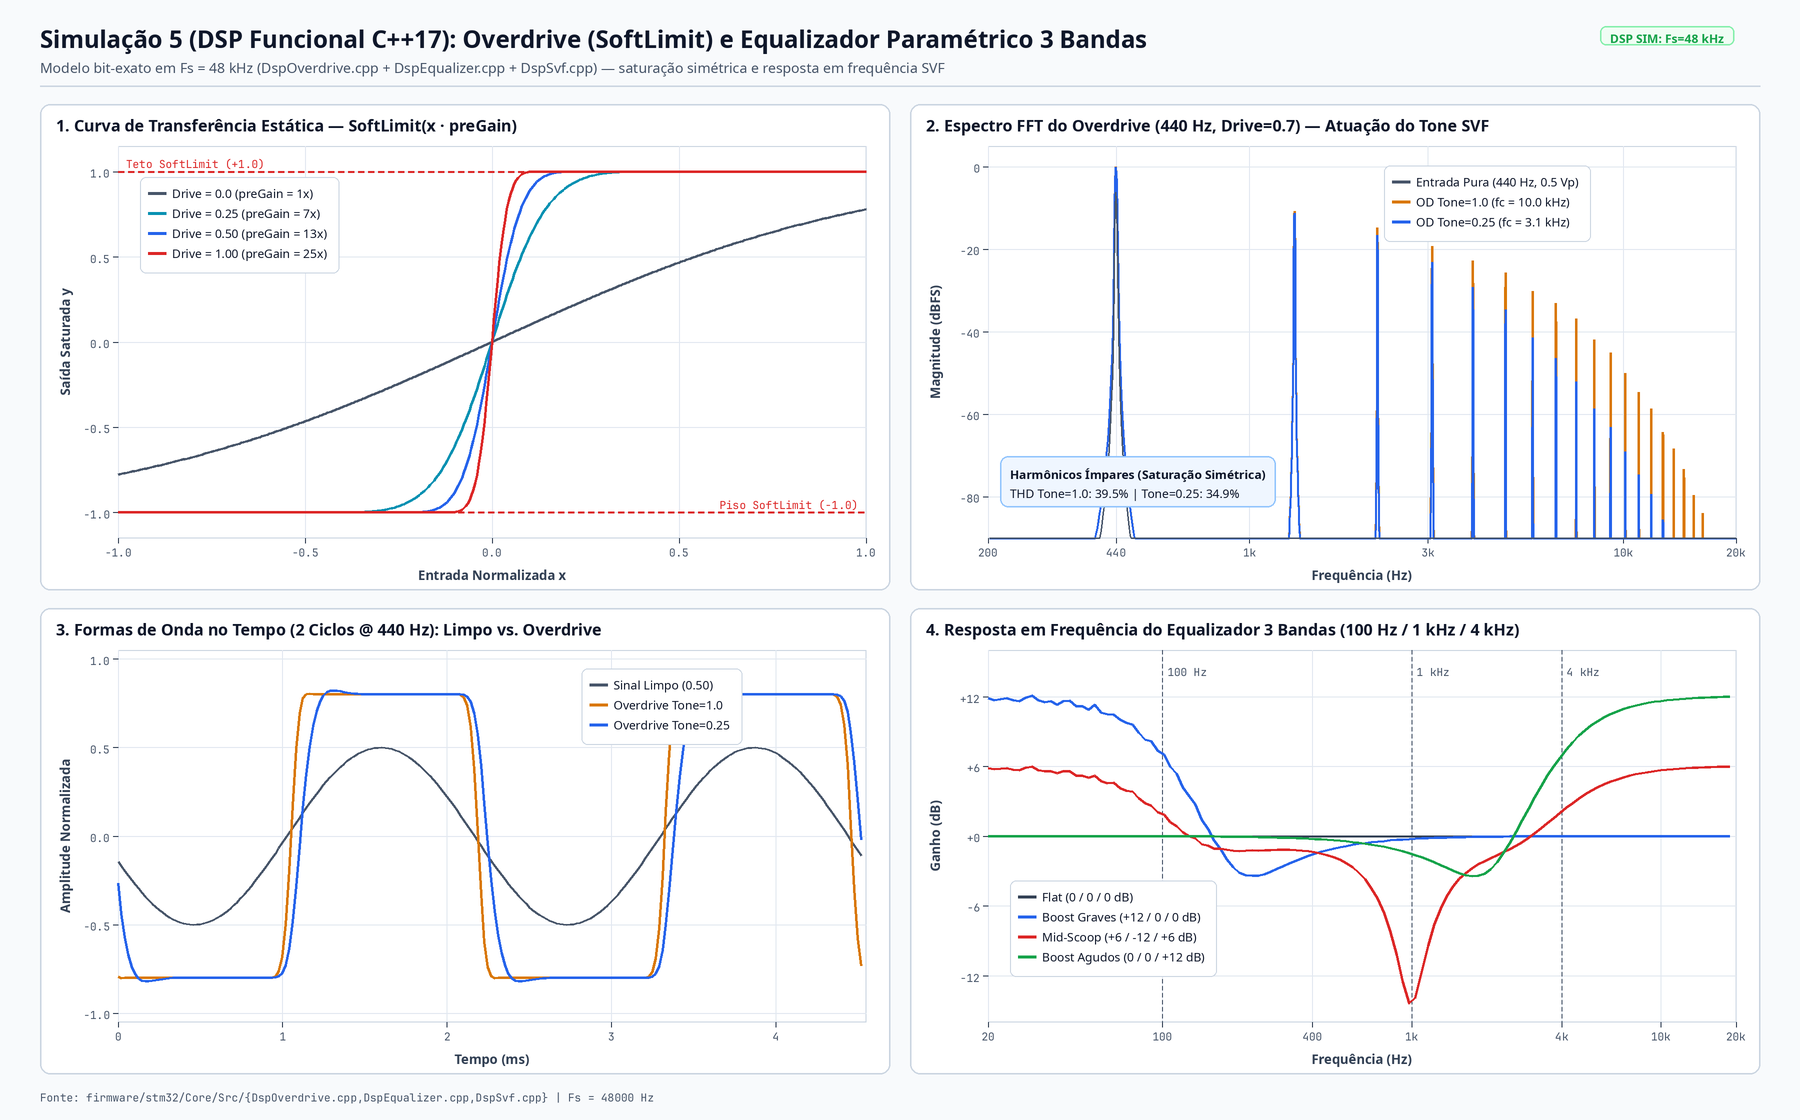
\includegraphics[width=0.88\textwidth]{figuras/sim5_dsp_overdrive_eq.png}
  \fonte{Elaborado pelos autores (2026).}\end{figure}
\begin{figure}[htbp]\centering\caption{Simulação DSP C++17: comparação entre chaveamento abrupto e \textit{crossfade} de potência constante.}\label{fig:sim6}
  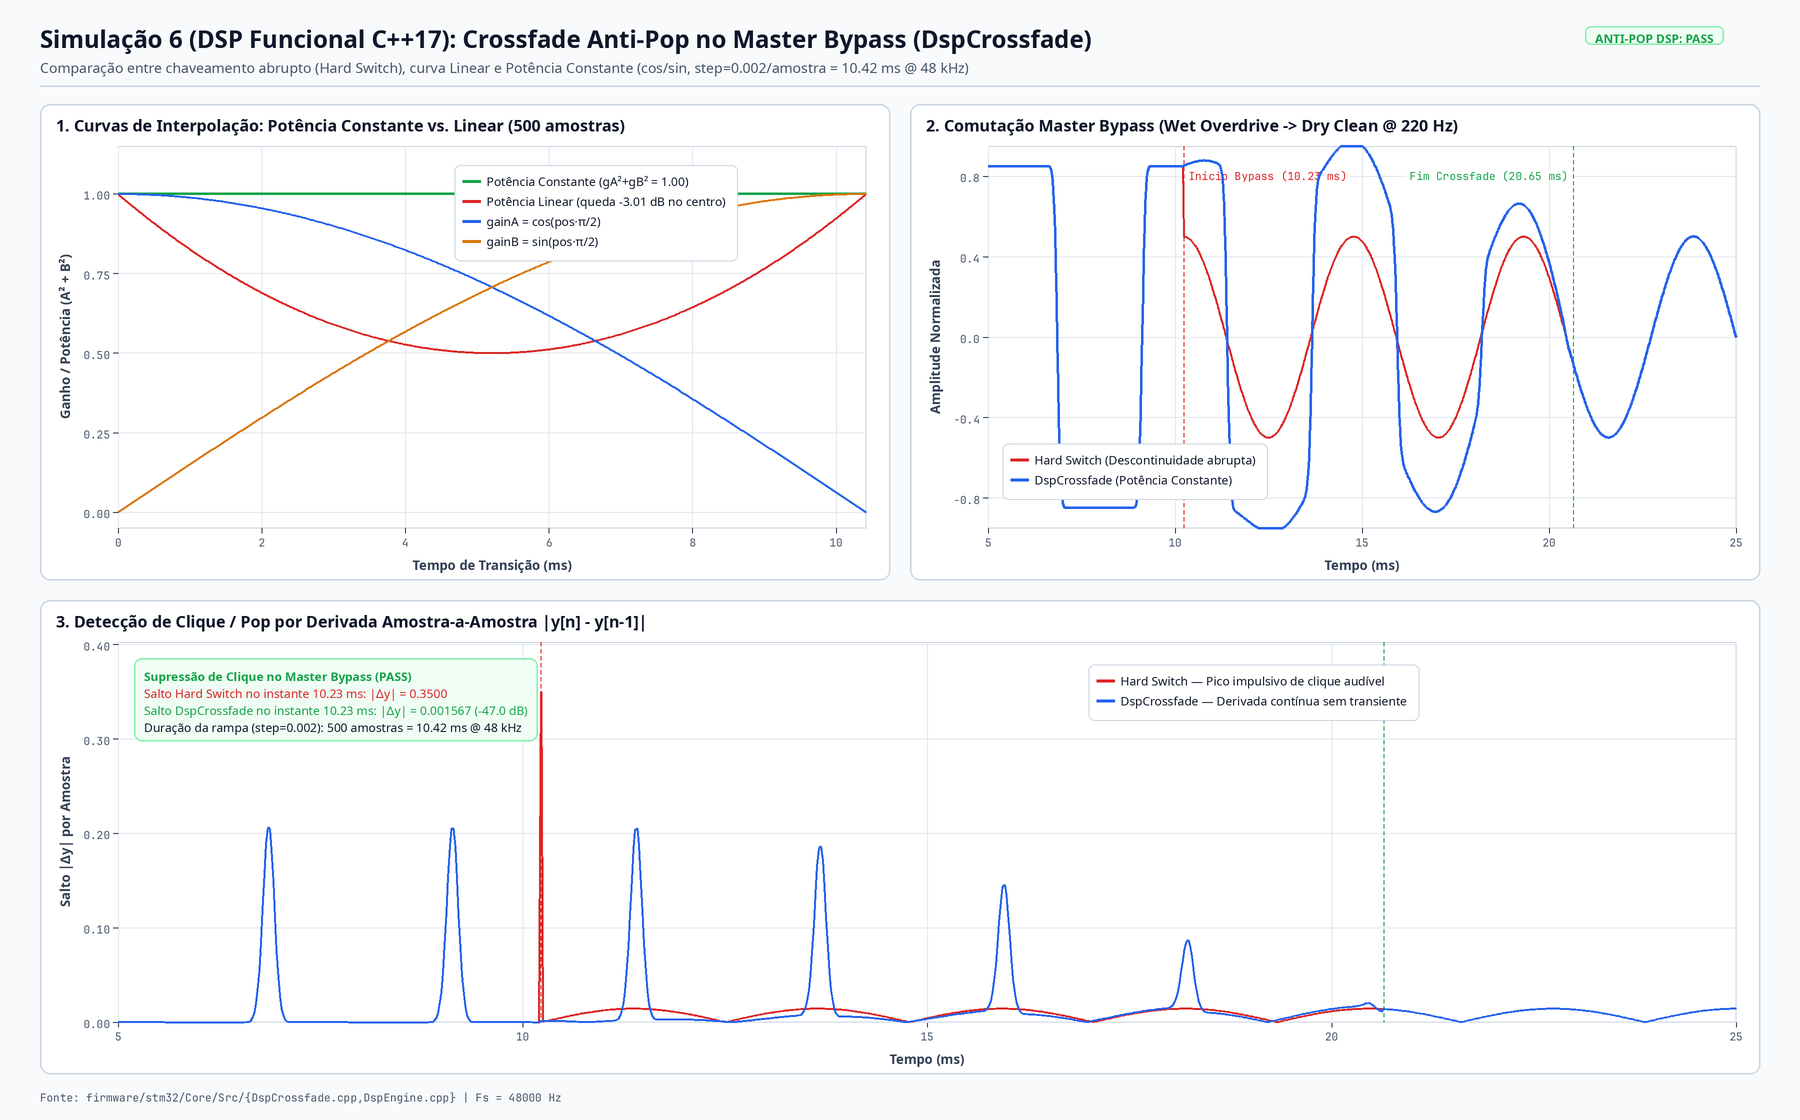
\includegraphics[width=0.88\textwidth]{figuras/sim6_dsp_crossfade_antipop.png}
  \fonte{Elaborado pelos autores (2026).}\end{figure}

\chapter{Gestão, Planejamento, Testes e Riscos}

\section{Orçamento Inicial}
A Tabela~\ref{tab:orcamento} estima o custo unitário integral (\textbf{R\$~518,50}) e o custo incremental a adquirir (\textbf{R\$~237,00}).
\begin{table}[htbp]\centering\caption{Orçamento inicial estimado da pedaleira digital.}\label{tab:orcamento}
  \footnotesize
  \setlength{\tabcolsep}{3.5pt}
  \begin{tabularx}{\textwidth}{C{0.7cm}Y C{0.9cm}C{1.5cm}C{1.5cm}L{1.7cm}L{2.1cm}}
    \toprule
    \textbf{Item} & \textbf{Descrição} & \textbf{Qtd.} & \textbf{Unit. (R\$)} & \textbf{Subtot. (R\$)} & \textbf{Situação} & \textbf{Referência} \\
    \midrule
    1 & Placa \texttt{WeAct STM32H723VG V1.2} & 1 & 145,00 & 145,00 & Em posse & AliExpress / ML \\
    2 & Módulo \texttt{ESP32 DevKit V1 (WROOM-32)} & 1 & 38,00 & 38,00 & Em posse & Varejo BR \\
    3 & Codec \texttt{CS4272} + Adaptador TSSOP-28 & 1 & 85,00 & 85,00 & Em posse & Distribuidor \\
    4 & Amp-Ops \texttt{TL072} (2x) + Regulador \texttt{CW7805} & 3 & 4,50 & 13,50 & Em posse & Comércio local \\
    5 & Fonte \texttt{12 V DC / 1,5 A} + Conector \texttt{J1} & 1 & 38,00 & 38,00 & Adquirir & Varejo BR \\
    6 & Isolador \texttt{ISO7721DR} + Adaptador DIP-8 & 1 & 24,00 & 24,00 & Adquirir & Distribuidor \\
    7 & Relé \texttt{Omron G5V-1-DC12} (\texttt{K1}) & 1 & 18,00 & 18,00 & Adquirir & Varejo BR \\
    8 & Referências \texttt{TL431ACZ} (2x) + Transistores/Diodos & 1 kit & 41,00 & 41,00 & Adquirir & Loja local \\
    9 & Chaves \texttt{MTS-102} (\texttt{SW1..4}) + LEDs (\texttt{D2..5}) & 4 cj. & 6,00 & 24,00 & Adquirir & Loja local \\
    10 & Conectores P10 (\texttt{J2, J3}), Borne e Pontos de Teste & 1 kit & 18,00 & 18,00 & Adquirir & Loja local \\
    11 & Lote Resistores $0{,}1\%$/$1\%$ e Capacitores & 1 kit & 50,00 & 50,00 & Adquirir & Varejo BR \\
    12 & Placa Perfurada Ilhada + Protoboard/Jumpers & 1 kit & 24,00 & 24,00 & Adquirir & Loja local \\
    \midrule
    \textbf{--} & \textbf{Custo Total Unitário / Incremental (Itens 5--12)} & \textbf{--} & \textbf{--} & \textbf{518,50 / 237,00} & \textbf{Resumo} & \textbf{--} \\
    \bottomrule
  \end{tabularx}
  \fonte{Elaborado pelos autores (2026).}
\end{table}

\section{Planejamento e Cronograma}
A Tabela~\ref{tab:cronograma} detalha o cronograma de 12 semanas conforme o andamento atual. Documentação, modelagem 3D, esquemáticos e simulações foram concluídos, enquanto a montagem física aguarda a compra dos insumos.
\begin{table}[htbp]\centering\caption{Planejamento e cronograma de desenvolvimento (12 semanas).}\label{tab:cronograma}
  \footnotesize
  \setlength{\tabcolsep}{3.5pt}
  \begin{tabularx}{\textwidth}{L{1.7cm}L{2.5cm}Y L{2.3cm}L{2.1cm}}
    \toprule
    \textbf{Período} & \textbf{Etapa} & \textbf{Descrição das Atividades} & \textbf{Responsável} & \textbf{Estado Atual} \\
    \midrule
    \textbf{Sem. 1--2} & Requisitos & Definição do problema, RF01--RF07, RNF01--RNF06 e escopo. & Toda a equipe & Concluído \\
    \textbf{Sem. 2--4} & Arquitetura/CAD & Esquemáticos KiCad (10 folhas, 0 ERC), modelo 3D e 33 SPICE. & Rodrigues / João & Concluído \\
    \textbf{Sem. 5--7} & Firmware e Web & Biblioteca DSP C++17, UART CRC-8, ponte MQTT e App Web. & João / Isabelle & Validado em host \\
    \textbf{Sem. 8} & Aquisição & Compra dos componentes discretos e eletromecânicos pendentes. & Arthur / Rodrigues & Pendente (insumos) \\
    \textbf{Sem. 9--10} & Bancada & Qualificação \texttt{CW7805}, protoboard e placa perfurada. & Toda a equipe & Não iniciada \\
    \textbf{Sem. 11} & Validação Física & Ensaios com guitarra, osciloscópio e reconfiguração Web/MQTT. & Toda a equipe & Não iniciada \\
    \textbf{Sem. 12} & Entrega & Consolidação dos requisitos, 3D, esquemáticos e simulações. & Toda a equipe & Concluído \\
    \bottomrule
  \end{tabularx}
  \fonte{Elaborado pelos autores (2026).}
\end{table}

\section{Estratégia de Prototipagem}
A prototipagem segue três ciclos incrementais (\textbf{V0, V1 e V2}), conforme a Figura~\ref{fig:prototipagem}.
\begin{figure}[htbp]
  \centering
  \caption{Estratégia incremental de prototipagem em três ciclos (V0, V1 e V2).}
  \label{fig:prototipagem}
  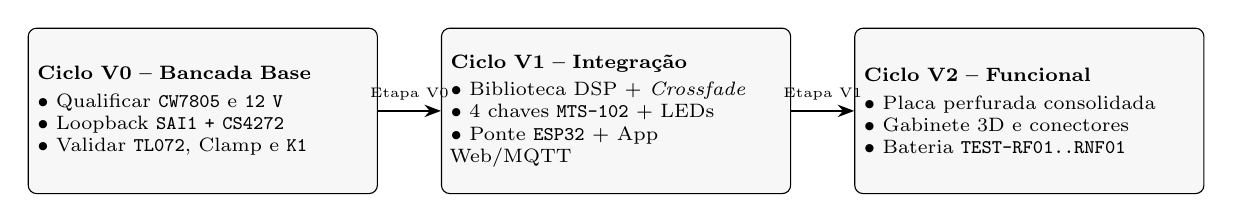
\begin{tikzpicture}[
    node distance=0.8cm,
    cycle/.style={rectangle, draw=black, rounded corners=3pt, text width=4.2cm, minimum height=2.1cm, align=left, font=\scriptsize, fill=gray!6},
    arr/.style={-{Stealth[scale=0.9]}, thick}
  ]
    \node[cycle] (v0) {\textbf{Ciclo V0 -- Bancada Base}\\[2pt]
      $\bullet$ Qualificar \texttt{CW7805} e \texttt{12 V}\\
      $\bullet$ Loopback \texttt{SAI1 + CS4272}\\
      $\bullet$ Validar \texttt{TL072}, Clamp e \texttt{K1}};
    \node[cycle, right=of v0] (v1) {\textbf{Ciclo V1 -- Integração}\\[2pt]
      $\bullet$ Biblioteca DSP + \textit{Crossfade}\\
      $\bullet$ 4 chaves \texttt{MTS-102} + LEDs\\
      $\bullet$ Ponte \texttt{ESP32} + App Web/MQTT};
    \node[cycle, right=of v1] (v2) {\textbf{Ciclo V2 -- Funcional}\\[2pt]
      $\bullet$ Placa perfurada consolidada\\
      $\bullet$ Gabinete 3D e conectores\\
      $\bullet$ Bateria \texttt{TEST-RF01..RNF01}};
    \draw[arr] (v0) -- node[above,font=\tiny]{Etapa V0} (v1);
    \draw[arr] (v1) -- node[above,font=\tiny]{Etapa V1} (v2);
  \end{tikzpicture}
  \fonte{Elaborado pelos autores (2026).}
\end{figure}

\section{Plano Inicial de Testes}
A Tabela~\ref{tab:testes} define os ensaios futuros em bancada para validação dos requisitos.
\begin{table}[htbp]\centering\caption{Plano inicial de testes experimentais em bancada.}\label{tab:testes}
  \footnotesize
  \setlength{\tabcolsep}{3.5pt}
  \begin{tabularx}{\textwidth}{L{1.8cm}C{1.1cm}Y L{3.6cm}L{3.5cm}}
    \toprule
    \textbf{ID Teste} & \textbf{Req.} & \textbf{Procedimento Experimental} & \textbf{Resultado Esperado} & \textbf{Critério de Aceite} \\
    \midrule
    \textbf{TEST-RF01} & \texttt{RF01} & Varredura $20\text{ Hz--}20\text{ kHz}$ em Overdrive, EQ e Delay. & Curvas fiéis e harmônicos controlados. & EQ $\pm 12\text{ dB}$; DSP $< 70\%$ DMA. \\
    \textbf{TEST-RF02} & \texttt{RF02} & Reatribuir efeitos em \texttt{SW1..SW3} e alternar \texttt{SW4}. & Chaves acionam o efeito mapeado com LED. & 100\% detecção sem repique. \\
    \textbf{TEST-RF03} & \texttt{RF03} & Alterar parâmetros via Web e desconectar Wi-Fi. & Sincronismo MQTT sem interromper áudio. & Atraso $\le 200\text{ ms}$; \texttt{0} cortes. \\
    \textbf{TEST-RF04} & \texttt{RF04} & Enviar 1.000 quadros UART via \texttt{ISO7721DR}. & Decodificação CRC-8 sem retorno USB. & Perda $< 0{,}1\%$; zero \textit{backpower}. \\
    \textbf{TEST-RF05} & \texttt{RF05} & Injetar senoide e sobrecarga em \texttt{J2}; medir \texttt{TP6..8}. & Limitação simétrica pelo clamp do ADC. & 48~kHz; $\text{THD} < 0{,}1\%$. \\
    \textbf{TEST-RF06} & \texttt{RF06} & Medir \texttt{J3} em \textit{bypass} no osciloscópio e FFT. & Resposta plana sem ruído de 60~Hz. & Ruído $< -80\text{ dBV}$; $\text{THD} < 0{,}05\%$. \\
    \textbf{TEST-RF07} & \texttt{RF07} & Medir \texttt{J3} ao comutar chaves e ligar/desligar 12~V. & Crossfade suave e aterramento por \texttt{K1}. & DSP $< -60\text{ dBFS}$; pop $< 5\text{ mV}$. \\
    \textbf{TEST-RNF01} & \texttt{RNF01} & Aplicar pulso em \texttt{J2} e medir atraso até \texttt{J3}. & Latência imperceptível ao vivo. & $\Delta t \le 10{,}0\text{ ms}$ (meta 4--7~ms). \\
    \bottomrule
  \end{tabularx}
  \fonte{Elaborado pelos autores (2026).}
\end{table}

\section{Riscos Técnicos}
A Tabela~\ref{tab:riscos} resume os riscos técnicos identificados e suas ações preventivas.
\begin{table}[htbp]\centering\caption{Matriz de riscos técnicos e estratégias de mitigação.}\label{tab:riscos}
  \footnotesize
  \setlength{\tabcolsep}{3.5pt}
  \begin{tabularx}{\textwidth}{C{0.9cm}L{3.7cm}C{1.5cm}L{2.4cm}Y}
    \toprule
    \textbf{ID} & \textbf{Risco Técnico} & \textbf{Sev./Prob.} & \textbf{Estado} & \textbf{Estratégia de Mitigação} \\
    \midrule
    \texttt{R01} & Indisponibilidade de insumos para bancada & Alta / Alta & Ativo & Entrega focada em requisitos, 3D, esquemáticos e simulações; montagem pós-aquisição. \\
    \texttt{R02} & Latência $> 10\text{ ms}$ ou \textit{overrun} de DMA & Média / Baixa & Monitorado & Blocos de 32--64 amostras, compilação \texttt{-O3} e FPU Cortex-M7. \\
    \texttt{R03} & Dessincronia entre Web/MQTT e chaves & Média / Média & Mitigado & Quadros UART com CRC-8 e chave \texttt{SW4} dedicada ao Modo Config. \\
    \texttt{R04} & Sobretensão ou retorno elétrico no codec & Alta / Média & Mitigado SPICE & Clamp ativo $V_{be}$, intertravamento \texttt{/RST} e isolador \texttt{ISO7721DR}. \\
    \texttt{R05} & Estalos na partida, troca ou queda de energia & Alta / Alta & Mitigado SPICE & Crossfade ($\cos/\sin$) + relé \texttt{K1} (\texttt{NC -> GND}) com \texttt{TL431}. \\
    \texttt{R06} & Pinagem do \texttt{CW7805} ou variante \texttt{ESP32} & Alta / Média & Pré-requisito & Qualificar \texttt{CW7805} com carga antes do codec e checar \texttt{GPIO16/17}. \\
    \texttt{R07} & Ruído 60~Hz ou mau contato em protoboard & Alta / Alta & Mitigado V2 & Placa perfurada soldada, terra em estrela e cabos P10 blindados. \\
    \bottomrule
  \end{tabularx}
  \fonte{Elaborado pelos autores (2026).}
\end{table}

\section{Organização da Equipe}
A Tabela~\ref{tab:equipe} define as responsabilidades dos integrantes \cite{ifpb2026roteiro}.
\begin{table}[htbp]\centering\caption{Organização da equipe e subsistemas associados.}\label{tab:equipe}
  \footnotesize
  \begin{tabularx}{\textwidth}{L{3.1cm}Y L{2.5cm}}
    \toprule
    \textbf{Integrante} & \textbf{Responsabilidades Principais} & \textbf{Subsistemas} \\
    \midrule
    \textbf{João Paulo} & Firmware DSP C++17 na \texttt{STM32H723VG} (biblioteca expansível, mapeamento dinâmico, \textit{crossfade}) e UART. & \texttt{SS01}, \texttt{SS02} \\
    \textbf{Isabelle Lavínia} & Firmware IoT no \texttt{ESP32} (Wi-Fi/MQTT), aplicação Web de configuração e documentação técnica. & \texttt{SS02}, \texttt{SS01} \\
    \textbf{Arthur Ramalho} & Integração do codec \texttt{CS4272}, painel físico (\texttt{SW1..SW4} e LEDs) e ensaios instrumentados. & \texttt{SS03}, \texttt{SS04}, \texttt{SS07} \\
    \textbf{Rodrigues Matheus} & Projeto elétrico, esquemáticos KiCad, simulações SPICE, alimentação/proteções e modelo 3D. & \texttt{SS05}, \texttt{SS06}, \texttt{SS07} \\
    \bottomrule
  \end{tabularx}
  \fonte{Elaborado pelos autores (2026).}
\end{table}

\section{Repositório do Projeto}
O código-fonte e a documentação encontram-se em \url{https://github.com/Rodriguesmath/Pedaleira-digital.git}:
\begin{verbatim}
Pedaleira-digital/
|-- docs/                     # Requisitos, escopo, protocolos e esquematicos
|-- firmware/                 # stm32/ (C++17 DSP) e esp32/ (ponte MQTT)
|-- app/                      # Aplicacao Web e servico MQTT de configuracao
|-- output/ENTREGA_DISCIPLINA/# Documentacao tecnica, renders 3D e simulacoes
`-- tests/                    # Testes unitarios e de integracao
\end{verbatim}

\section{Registro do Desenvolvimento e Próximos Passos}
Até novembro de 2026, o projeto entregou o esquemático no KiCad 10 em 10 folhas (183 componentes, 96 redes e \textbf{zero erros ERC}) e \textbf{33 simulações SPICE aprovadas} em \texttt{ngspice}. No mesmo período, a equipe concluiu a biblioteca DSP em C++17 (\textit{Overdrive}, EQ 3 bandas, \textit{Delay}, \textit{Crossfade}), o protocolo UART CRC-8, a ponte \texttt{ESP32}/MQTT, a aplicação Web e o gabinete 3D (\texttt{.stl}). \textbf{Nenhuma montagem física em bancada foi realizada até o momento} por indisponibilidade de insumos. Toda validação atual apoia-se em projeto, modelagem 3D e simulações.

Os próximos passos incluem a aquisição dos componentes pendentes, a qualificação isolada do regulador \texttt{CW7805}, a montagem progressiva \texttt{V0 -> V1 -> V2} e a execução da bateria experimental \texttt{TEST-RF01..RNF01} com instrumento real e reconfiguração Web/MQTT.

\section{Checklist para Entrega}
A Tabela~\ref{tab:checklist} verifica os 23 critérios da Seção 32 do Roteiro IFPB \cite{ifpb2026roteiro}.
\begin{table}[htbp]\centering\caption{Checklist de conformidade com o Roteiro de Entrega IFPB (\S32).}\label{tab:checklist}
  \scriptsize
  \setlength{\tabcolsep}{3.5pt}
  \renewcommand{\arraystretch}{1.02}
  \begin{tabularx}{\textwidth}{C{0.7cm}Y C{1.3cm}L{5.2cm}}
    \toprule
    \textbf{\#} & \textbf{Critério Obrigatório do Roteiro IFPB} & \textbf{Status} & \textbf{Evidência / Localização} \\
    \midrule
    1 & O nome do projeto foi definido? & [X] Sim & \texttt{PED-DIGITAL}, Tabela~\ref{tab:identificacao}. \\
    2 & O problema está claramente explicado? & [X] Sim & Tabela~\ref{tab:problema} e Pergunta de Projeto. \\
    3 & A justificativa está fundamentada? & [X] Sim & Capítulo 1, Seção 1.4. \\
    4 & O público-alvo foi identificado? & [X] Sim & Tabela~\ref{tab:publico}. \\
    5 & O objetivo geral está definido? & [X] Sim & Capítulo 1, Seção 1.7. \\
    6 & Os objetivos específicos foram definidos? & [X] Sim & Capítulo 1, Seção 1.8. \\
    7 & Os requisitos funcionais foram especificados? & [X] Sim & Tabela~\ref{tab:rf} (\texttt{RF01..RF07}). \\
    8 & Os requisitos não funcionais foram especificados? & [X] Sim & Tabela~\ref{tab:rnf} (\texttt{RNF01..RNF06}). \\
    9 & O escopo positivo foi definido? & [X] Sim & Capítulo 2, Seção 2.3. \\
    10 & O escopo negativo foi definido? & [X] Sim & Capítulo 2, Seção 2.4. \\
    11 & Existe um diagrama conceitual? & [X] Sim & Figura~\ref{fig:conceitual}. \\
    12 & Existe uma arquitetura preliminar? & [X] Sim & Figura~\ref{fig:arquitetura}. \\
    13 & O projeto foi dividido em subsistemas? & [X] Sim & Tabela~\ref{tab:subsistemas} (\texttt{SS01..SS07}). \\
    14 & Os principais componentes foram selecionados? & [X] Sim & Tabela~\ref{tab:bom} (183 itens). \\
    15 & A escolha dos componentes foi justificada? & [X] Sim & Capítulo 3, Seção 3.4. \\
    16 & Os datasheets foram consultados? & [X] Sim & Tabela~\ref{tab:datasheets}. \\
    17 & Existe uma estimativa de custo? & [X] Sim & Tabela~\ref{tab:orcamento} (R\$~518,50 / R\$~237,00). \\
    18 & Existe um cronograma? & [X] Sim & Tabela~\ref{tab:cronograma} (12 semanas). \\
    19 & Existem responsáveis pelas atividades? & [X] Sim & Tabelas~\ref{tab:subsistemas}, \ref{tab:cronograma} e \ref{tab:equipe}. \\
    20 & Existe uma estratégia de prototipagem? & [X] Sim & Figura~\ref{fig:prototipagem} (\texttt{V0}, \texttt{V1}, \texttt{V2}). \\
    21 & Existe um plano inicial de testes? & [X] Sim & Tabela~\ref{tab:testes} (\texttt{TEST-RF01..RNF01}). \\
    22 & Os principais riscos foram identificados? & [X] Sim & Tabela~\ref{tab:riscos} (\texttt{R01..R07}). \\
    23 & O repositório Git foi criado? & [X] Sim & Capítulo 6, Seção 6.7. \\
    \bottomrule
  \end{tabularx}
  \fonte{Elaborado pelos autores com base em \citeonline{ifpb2026roteiro} (2026).}
\end{table}

% ==============================================================================
% ELEMENTOS POS-TEXTUAIS
% ==============================================================================
\postextual

\bibliography{referencias}

\begin{anexosenv}
\partanexos

\chapter{Esquemático Elétrico Completo (10 Folhas KiCad)}
Este anexo reúne as 10 folhas esquemáticas geradas no KiCad 10 com zero violações ERC. O conjunto inclui alimentação e supervisão, estágio analógico de entrada com clamp ativo do ADC, codec \texttt{CS4272}, saída com relé \textit{anti-pop}, \texttt{STM32H723VG}, isolador UART \texttt{ISO7721DR}, módulo \texttt{ESP32}, chaves físicas e pontos de teste.

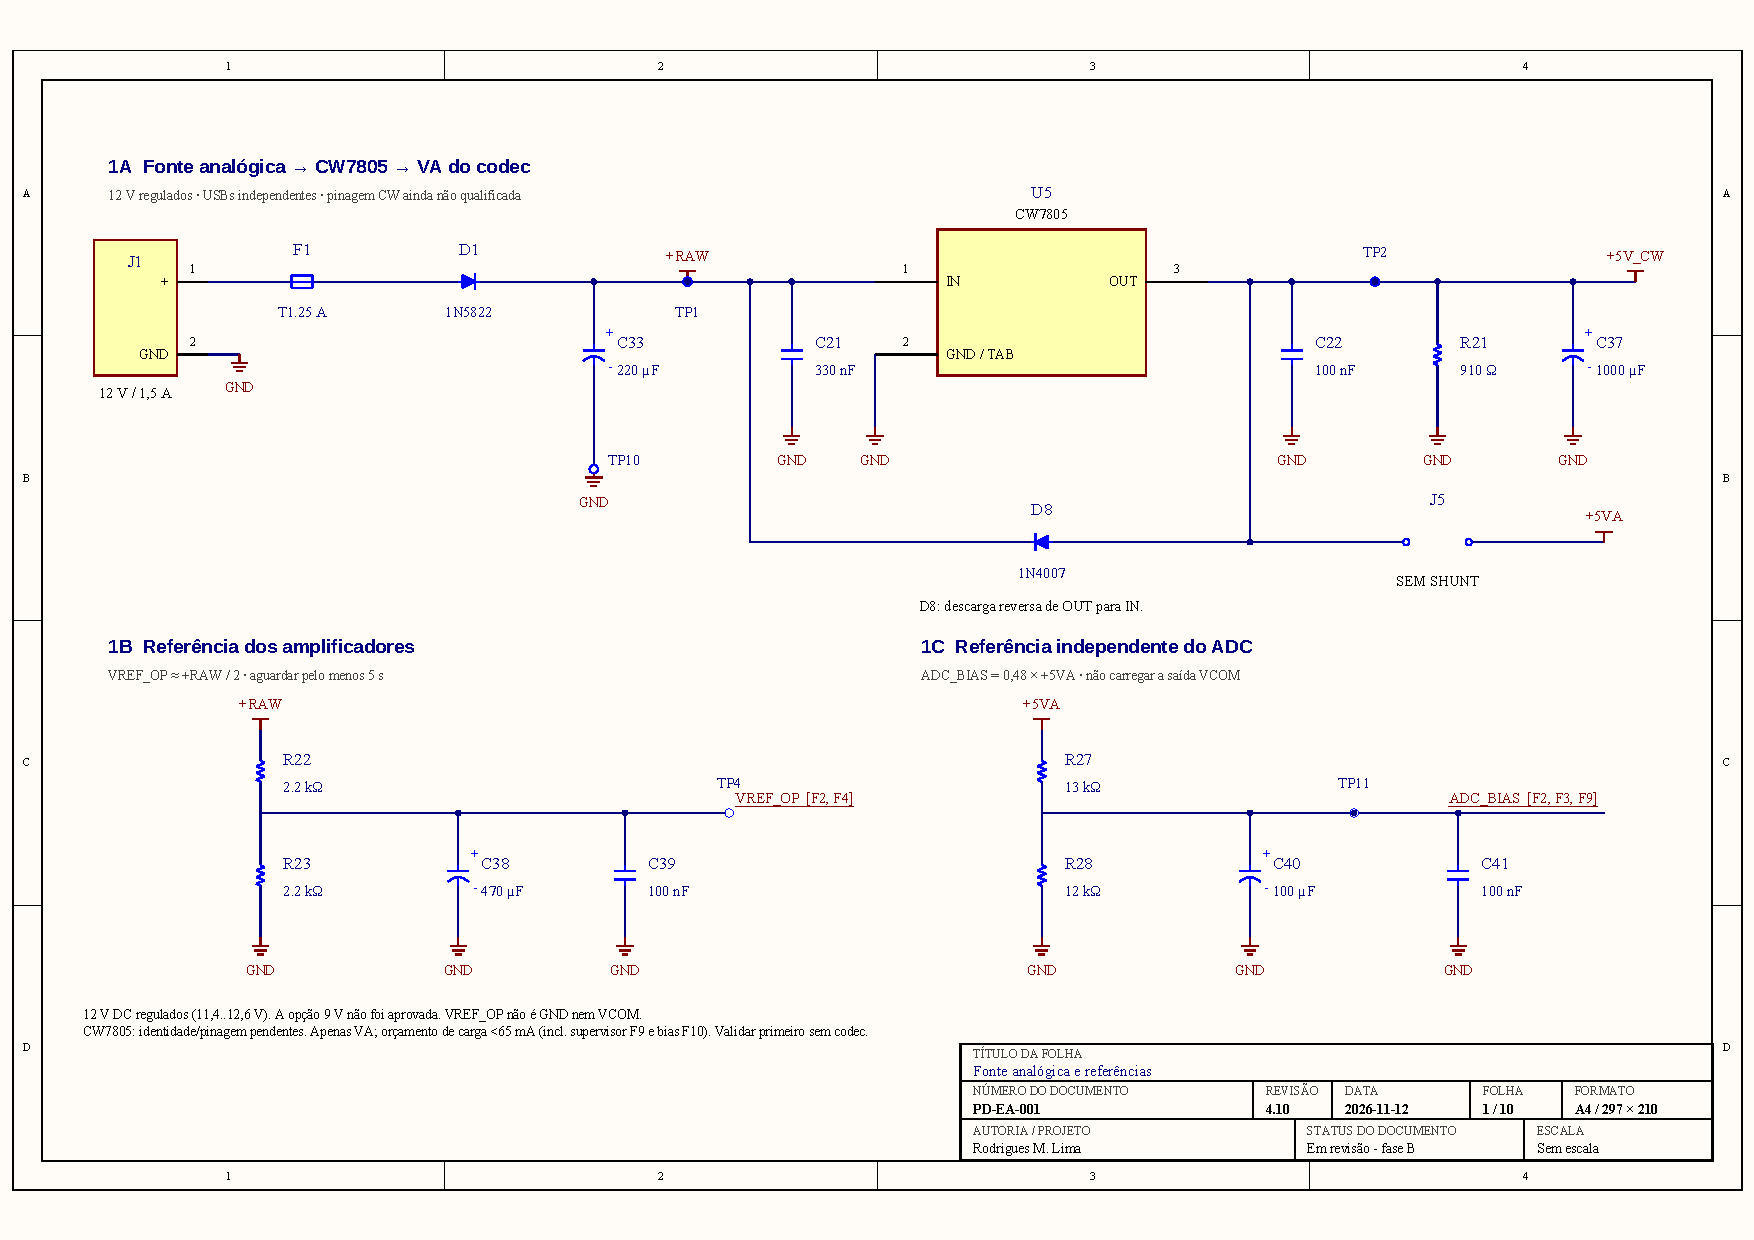
\includepdf[pages=-,pagecommand={\thispagestyle{abntheadings}}]{figuras/pedaleira_digital_rev4_10_esquematico.pdf}

\end{anexosenv}

\end{document}
